% Options for packages loaded elsewhere
% Options for packages loaded elsewhere
\PassOptionsToPackage{unicode}{hyperref}
\PassOptionsToPackage{hyphens}{url}
\PassOptionsToPackage{dvipsnames,svgnames,x11names}{xcolor}
%
\documentclass[
  french,
  11pt,
  a4paper,
]{article}
\usepackage{xcolor}
\usepackage[a4paper,textheight=24cm,textwidth=15.5cm]{geometry}
\usepackage{amsmath,amssymb}
\setcounter{secnumdepth}{5}
\usepackage{iftex}
\ifPDFTeX
  \usepackage[T1]{fontenc}
  \usepackage[utf8]{inputenc}
  \usepackage{textcomp} % provide euro and other symbols
\else % if luatex or xetex
  \usepackage{unicode-math} % this also loads fontspec
  \defaultfontfeatures{Scale=MatchLowercase}
  \defaultfontfeatures[\rmfamily]{Ligatures=TeX,Scale=1}
\fi
\usepackage[]{montserrat}
\ifPDFTeX\else
  % xetex/luatex font selection
  \setmonofont[Scale=0.92]{montserrat}
\fi
% Use upquote if available, for straight quotes in verbatim environments
\IfFileExists{upquote.sty}{\usepackage{upquote}}{}
\IfFileExists{microtype.sty}{% use microtype if available
  \usepackage[]{microtype}
  \UseMicrotypeSet[protrusion]{basicmath} % disable protrusion for tt fonts
}{}
\makeatletter
\@ifundefined{KOMAClassName}{% if non-KOMA class
  \IfFileExists{parskip.sty}{%
    \usepackage{parskip}
  }{% else
    \setlength{\parindent}{0pt}
    \setlength{\parskip}{6pt plus 2pt minus 1pt}}
}{% if KOMA class
  \KOMAoptions{parskip=half}}
\makeatother
% Make \paragraph and \subparagraph free-standing
\makeatletter
\ifx\paragraph\undefined\else
  \let\oldparagraph\paragraph
  \renewcommand{\paragraph}{
    \@ifstar
      \xxxParagraphStar
      \xxxParagraphNoStar
  }
  \newcommand{\xxxParagraphStar}[1]{\oldparagraph*{#1}\mbox{}}
  \newcommand{\xxxParagraphNoStar}[1]{\oldparagraph{#1}\mbox{}}
\fi
\ifx\subparagraph\undefined\else
  \let\oldsubparagraph\subparagraph
  \renewcommand{\subparagraph}{
    \@ifstar
      \xxxSubParagraphStar
      \xxxSubParagraphNoStar
  }
  \newcommand{\xxxSubParagraphStar}[1]{\oldsubparagraph*{#1}\mbox{}}
  \newcommand{\xxxSubParagraphNoStar}[1]{\oldsubparagraph{#1}\mbox{}}
\fi
\makeatother

\usepackage{color}
\usepackage{fancyvrb}
\newcommand{\VerbBar}{|}
\newcommand{\VERB}{\Verb[commandchars=\\\{\}]}
\DefineVerbatimEnvironment{Highlighting}{Verbatim}{commandchars=\\\{\}}
% Add ',fontsize=\small' for more characters per line
\newenvironment{Shaded}{}{}
\newcommand{\AlertTok}[1]{\textcolor[rgb]{1.00,0.33,0.33}{\textbf{#1}}}
\newcommand{\AnnotationTok}[1]{\textcolor[rgb]{0.42,0.45,0.49}{#1}}
\newcommand{\AttributeTok}[1]{\textcolor[rgb]{0.84,0.23,0.29}{#1}}
\newcommand{\BaseNTok}[1]{\textcolor[rgb]{0.00,0.36,0.77}{#1}}
\newcommand{\BuiltInTok}[1]{\textcolor[rgb]{0.84,0.23,0.29}{#1}}
\newcommand{\CharTok}[1]{\textcolor[rgb]{0.01,0.18,0.38}{#1}}
\newcommand{\CommentTok}[1]{\textcolor[rgb]{0.42,0.45,0.49}{#1}}
\newcommand{\CommentVarTok}[1]{\textcolor[rgb]{0.42,0.45,0.49}{#1}}
\newcommand{\ConstantTok}[1]{\textcolor[rgb]{0.00,0.36,0.77}{#1}}
\newcommand{\ControlFlowTok}[1]{\textcolor[rgb]{0.84,0.23,0.29}{#1}}
\newcommand{\DataTypeTok}[1]{\textcolor[rgb]{0.84,0.23,0.29}{#1}}
\newcommand{\DecValTok}[1]{\textcolor[rgb]{0.00,0.36,0.77}{#1}}
\newcommand{\DocumentationTok}[1]{\textcolor[rgb]{0.42,0.45,0.49}{#1}}
\newcommand{\ErrorTok}[1]{\textcolor[rgb]{1.00,0.33,0.33}{\underline{#1}}}
\newcommand{\ExtensionTok}[1]{\textcolor[rgb]{0.84,0.23,0.29}{\textbf{#1}}}
\newcommand{\FloatTok}[1]{\textcolor[rgb]{0.00,0.36,0.77}{#1}}
\newcommand{\FunctionTok}[1]{\textcolor[rgb]{0.44,0.26,0.76}{#1}}
\newcommand{\ImportTok}[1]{\textcolor[rgb]{0.01,0.18,0.38}{#1}}
\newcommand{\InformationTok}[1]{\textcolor[rgb]{0.42,0.45,0.49}{#1}}
\newcommand{\KeywordTok}[1]{\textcolor[rgb]{0.84,0.23,0.29}{#1}}
\newcommand{\NormalTok}[1]{\textcolor[rgb]{0.14,0.16,0.18}{#1}}
\newcommand{\OperatorTok}[1]{\textcolor[rgb]{0.14,0.16,0.18}{#1}}
\newcommand{\OtherTok}[1]{\textcolor[rgb]{0.44,0.26,0.76}{#1}}
\newcommand{\PreprocessorTok}[1]{\textcolor[rgb]{0.84,0.23,0.29}{#1}}
\newcommand{\RegionMarkerTok}[1]{\textcolor[rgb]{0.42,0.45,0.49}{#1}}
\newcommand{\SpecialCharTok}[1]{\textcolor[rgb]{0.00,0.36,0.77}{#1}}
\newcommand{\SpecialStringTok}[1]{\textcolor[rgb]{0.01,0.18,0.38}{#1}}
\newcommand{\StringTok}[1]{\textcolor[rgb]{0.01,0.18,0.38}{#1}}
\newcommand{\VariableTok}[1]{\textcolor[rgb]{0.89,0.38,0.04}{#1}}
\newcommand{\VerbatimStringTok}[1]{\textcolor[rgb]{0.01,0.18,0.38}{#1}}
\newcommand{\WarningTok}[1]{\textcolor[rgb]{1.00,0.33,0.33}{#1}}

\usepackage{longtable,booktabs,array}
\newcounter{none} % for unnumbered tables
\usepackage{calc} % for calculating minipage widths
% Correct order of tables after \paragraph or \subparagraph
\usepackage{etoolbox}
\makeatletter
\patchcmd\longtable{\par}{\if@noskipsec\mbox{}\fi\par}{}{}
\makeatother
% Allow footnotes in longtable head/foot
\IfFileExists{footnotehyper.sty}{\usepackage{footnotehyper}}{\usepackage{footnote}}
\makesavenoteenv{longtable}
\usepackage{graphicx}
\makeatletter
\newsavebox\pandoc@box
\newcommand*\pandocbounded[1]{% scales image to fit in text height/width
  \sbox\pandoc@box{#1}%
  \Gscale@div\@tempa{\textheight}{\dimexpr\ht\pandoc@box+\dp\pandoc@box\relax}%
  \Gscale@div\@tempb{\linewidth}{\wd\pandoc@box}%
  \ifdim\@tempb\p@<\@tempa\p@\let\@tempa\@tempb\fi% select the smaller of both
  \ifdim\@tempa\p@<\p@\scalebox{\@tempa}{\usebox\pandoc@box}%
  \else\usebox{\pandoc@box}%
  \fi%
}
% Set default figure placement to htbp
\def\fps@figure{htbp}
\makeatother


% definitions for citeproc citations
\NewDocumentCommand\citeproctext{}{}
\NewDocumentCommand\citeproc{mm}{%
  \begingroup\def\citeproctext{#2}\cite{#1}\endgroup}
\makeatletter
 % allow citations to break across lines
 \let\@cite@ofmt\@firstofone
 % avoid brackets around text for \cite:
 \def\@biblabel#1{}
 \def\@cite#1#2{{#1\if@tempswa , #2\fi}}
\makeatother
\newlength{\cslhangindent}
\setlength{\cslhangindent}{1.5em}
\newlength{\csllabelwidth}
\setlength{\csllabelwidth}{3em}
\newenvironment{CSLReferences}[2] % #1 hanging-indent, #2 entry-spacing
 {\begin{list}{}{%
  \setlength{\itemindent}{0pt}
  \setlength{\leftmargin}{0pt}
  \setlength{\parsep}{0pt}
  % turn on hanging indent if param 1 is 1
  \ifodd #1
   \setlength{\leftmargin}{\cslhangindent}
   \setlength{\itemindent}{-1\cslhangindent}
  \fi
  % set entry spacing
  \setlength{\itemsep}{#2\baselineskip}}}
 {\end{list}}
\usepackage{calc}
\newcommand{\CSLBlock}[1]{\hfill\break\parbox[t]{\linewidth}{\strut\ignorespaces#1\strut}}
\newcommand{\CSLLeftMargin}[1]{\parbox[t]{\csllabelwidth}{\strut#1\strut}}
\newcommand{\CSLRightInline}[1]{\parbox[t]{\linewidth - \csllabelwidth}{\strut#1\strut}}
\newcommand{\CSLIndent}[1]{\hspace{\cslhangindent}#1}

\ifLuaTeX
\usepackage[bidi=basic,shorthands=off]{babel}
\else
\usepackage[bidi=default,shorthands=off]{babel}
\fi
\ifLuaTeX
  \usepackage{selnolig} % disable illegal ligatures
\fi


\setlength{\emergencystretch}{3em} % prevent overfull lines

\providecommand{\tightlist}{%
  \setlength{\itemsep}{0pt}\setlength{\parskip}{0pt}}



 


\usepackage{tikz}
\usepackage{xcolor}
\usepackage{tabularx}
\usepackage{orcidlink}
\usepackage{lineno}
\usepackage{libertinus}
\usepackage{montserrat}
\usepackage{draftwatermark}

\usepackage{booktabs}
\usepackage{longtable}
\usepackage{array}
\usepackage{multirow}
\usepackage{wrapfig}
\usepackage{float}
\usepackage{colortbl}
\usepackage{pdflscape}
\usepackage{tabularx}
\usepackage{xltabular}
\usepackage{threeparttable}
\usepackage{threeparttablex}
\usepackage[normalem]{ulem}
\usepackage{makecell}
\usepackage{xcolor}
\makeatletter
\@ifpackageloaded{tcolorbox}{}{\usepackage[skins,breakable]{tcolorbox}}
\@ifpackageloaded{fontawesome5}{}{\usepackage{fontawesome5}}
\definecolor{quarto-callout-color}{HTML}{909090}
\definecolor{quarto-callout-note-color}{HTML}{0758E5}
\definecolor{quarto-callout-important-color}{HTML}{CC1914}
\definecolor{quarto-callout-warning-color}{HTML}{EB9113}
\definecolor{quarto-callout-tip-color}{HTML}{00A047}
\definecolor{quarto-callout-caution-color}{HTML}{FC5300}
\definecolor{quarto-callout-color-frame}{HTML}{acacac}
\definecolor{quarto-callout-note-color-frame}{HTML}{4582ec}
\definecolor{quarto-callout-important-color-frame}{HTML}{d9534f}
\definecolor{quarto-callout-warning-color-frame}{HTML}{f0ad4e}
\definecolor{quarto-callout-tip-color-frame}{HTML}{02b875}
\definecolor{quarto-callout-caution-color-frame}{HTML}{fd7e14}
\makeatother
\makeatletter
\@ifpackageloaded{caption}{}{\usepackage{caption}}
\AtBeginDocument{%
\ifdefined\contentsname
  \renewcommand*\contentsname{Table des matières}
\else
  \newcommand\contentsname{Table des matières}
\fi
\ifdefined\listfigurename
  \renewcommand*\listfigurename{Liste des Figures}
\else
  \newcommand\listfigurename{Liste des Figures}
\fi
\ifdefined\listtablename
  \renewcommand*\listtablename{Liste des Tables}
\else
  \newcommand\listtablename{Liste des Tables}
\fi
\ifdefined\figurename
  \renewcommand*\figurename{Figure}
\else
  \newcommand\figurename{Figure}
\fi
\ifdefined\tablename
  \renewcommand*\tablename{Table}
\else
  \newcommand\tablename{Table}
\fi
}
\@ifpackageloaded{float}{}{\usepackage{float}}
\floatstyle{ruled}
\@ifundefined{c@chapter}{\newfloat{codelisting}{h}{lop}}{\newfloat{codelisting}{h}{lop}[chapter]}
\floatname{codelisting}{Listing}
\newcommand*\listoflistings{\listof{codelisting}{Liste des Listings}}
\makeatother
\makeatletter
\makeatother
\makeatletter
\@ifpackageloaded{caption}{}{\usepackage{caption}}
\@ifpackageloaded{subcaption}{}{\usepackage{subcaption}}
\makeatother
\usepackage{bookmark}
\IfFileExists{xurl.sty}{\usepackage{xurl}}{} % add URL line breaks if available
\urlstyle{same}
\hypersetup{
  pdftitle={Identifier des facteurs latents en SHS},
  pdfauthor={Grégoire Le Campion; Solenne Roux},
  pdflang={fr-FR},
  pdfkeywords={Analyses factorielles, Analyses en composantes
principales, Facteurs latents},
  colorlinks=true,
  linkcolor={blue},
  filecolor={Maroon},
  citecolor={Blue},
  urlcolor={Blue},
  pdfcreator={LaTeX via pandoc}}


\title{Identifier des facteurs latents en SHS}
\usepackage{etoolbox}
\makeatletter
\providecommand{\subtitle}[1]{% add subtitle to \maketitle
  \apptocmd{\@title}{\par {\large #1 \par}}{}{}
}
\makeatother
\subtitle{Exemples d'application sur des données en Géographie en
utilisant le couple analyse factorielle exploratoire (EFA) / analyse
factorielle confirmatoire (CFA)}
\author{Grégoire Le Campion \and Solenne Roux}
\date{20 novembre 2026}
\begin{document}
\definecolor{rzine-blue}{HTML}{0C3762}
\definecolor{title-blue}{HTML}{C4D6EE}
\definecolor{title-grey}{HTML}{708090}



\begin{tikzpicture}[remember picture,overlay]
\fill[rzine-blue]
  (current page.north west) -- (current page.north east) --
  ([yshift=-5cm]current page.north east|-current page.north east) --
  ([yshift=-5cm]current page.north west|-current page.north west) -- cycle;
\node[anchor=north west, xshift=.75cm,
  yshift=-.75cm] at (current page.north west) {\includegraphics[height=3cm]{logo}};

\node[font=\sffamily\bfseries\color{title-blue},anchor=west,
  xshift=4.25cm,yshift=-2.3cm] at (current page.north west)
  {\begin{minipage}{15cm}
    \fontsize{22}{30}\selectfont
    Identifier des facteurs latents en SHS
    \vspace{.18cm}
    \\
    \fontsize{13}{18}\selectfont
    Exemples d'application sur des données en Géographie en utilisant le
    couple analyse factorielle exploratoire (EFA) / analyse factorielle
    confirmatoire (CFA)
    \vspace{.5cm}
    \\
    \fontsize{10}{18}\color{title-grey}\selectfont {\includegraphics[height=0.35cm]{cc-by}} ISSN 2743-8791 - Rzine.fr - Revue de méthodes pour les SHS  
    
  \end{minipage}};
\end{tikzpicture}

\vspace*{2.5cm}
\begin{center}
          Grégoire Le Campion~\orcidlink{0000-0001-7195-765X}\quad
             UMR Passages, CNRS\\
                 Solenne Roux~\orcidlink{0000-0002-5044-0608}\quad
             LabPsy, Université de Bordeaux\\
           
  \bigskip
  
  Date de publication: 20 novembre 2026
\end{center}
      
\bigskip
\begin{abstract}
Cet article présente deux méthodes d'analyse factorielle et leurs
applications sous R. Ces méthodes cousines de l'analyse en composante
principale, s'en distinguent notamment car elles permettent de mettre en
évidence des facteurs latents plutôt que des composantes principales.
Cette approche par les facteurs latents est surtout utilisée en
Psychologie. Moins répandue dans les autres disciplines des sciences
humaines et sociales, elle pourrait néanmoins s'avérer particulièrement
utile pour répondre à des hypothèses ou besoins particuliers dans toutes
les disciplines des SHS. \textbf{Pré-requis} : Connaissances de base en
traitement et analyse de données. Être familier des risques induits par
les outliers, la multicolinéarité, etc. dans la modélisation
statistique.
\end{abstract}

\noindent%
{\it Keywords:} Analyses factorielles, Analyses en composantes
principales, Facteurs latents
\vfill

\DraftwatermarkOptions{stamp=false}

\renewcommand*\contentsname{Table des matières}
{
\setcounter{tocdepth}{3}
\tableofcontents
}
\listoffigures
\listoftables

\section*{Introduction}\label{introduction}
\addcontentsline{toc}{section}{Introduction}

\section{L'analyse factorielle}\label{lanalyse-factorielle}

\emph{Comment rendre compte, de manière simple, de la complexité des
différents types de relations qui existent entre plusieurs variables
d'une base de données ?}

C'est à cette question que permet, entre autres, de répondre l'analyse
multivariée, et par extension les méthodes d'analyse factorielle qui
appartiennent à ce champ de méthodes.

\subsection{L'Objectif de l'analyse factorielle
?}\label{lobjectif-de-lanalyse-factorielle}

L'objectif général de l'analyse factorielle est de réduire un nombre
important d'informations (c'est-à-dire les valeurs contenues dans
différentes variables) à quelques grandes dimensions. Il s'agit de
synthétiser l'information. Par exemple, imaginons des chercheurs
souhaitant étudier le comportement de préservation de l'environnement
des français. Pour cela, ils récoltent différentes données concernant le
statut socioprofessionnel des participants, leur état de santé, leur
zone géographique d'habitation, leur implication dans des associations,
etc. Ils recueillent donc beaucoup de données dans chacun des différents
thèmes susceptibles d'expliquer leurs hypothèses. Afin de synthétiser
l'information alors recueillie, et éventuellement par la suite de
pouvoir dégager des profils de comportement ou des liens de causalité,
ils feront d'abord appel à l'une des méthodes de factorisation
existantes.

Comme dans toute analyse statistique, on va chercher à expliquer la plus
forte proportion de la variance (de la covariance dans le cas de
l'analyse factorielle) par un nombre aussi restreint que possible de
variables (appelées dans l'analyse factorielle composantes ou facteurs).

\subsection{Les différents types d'analyses
factorielles}\label{les-diffuxe9rents-types-danalyses-factorielles}

Ce que nous appelons communément \emph{Analyses Factorielles} rassemble
différentes méthodes qui se répartissent en deux grandes familles
(cf.~Tabachnick \& Fidell - 6ème ed 2014).

Les premiers à théoriser les méthodes d'analyses factorielles sont le
mathématicien britannique Karl Pearson (1901) et le psychologue anglais
Charles Spearman (1904). Pearson développera sa réflexion sur les
\emph{Analyses en Composantes Principales (ACP)} (Pearson F.R.S., K.,
1901). Alors que Spearman se concentrera sur l'\emph{Analyse
Factorielle}, afin de rendre compte de la variance commune partagée par
les items d'un même outil psychométrique (Spearman, C., 1904).

Ces pionniers des analyses factorielles travaillaient déjà sur les
corrélations, et ce sont ces mêmes personnes qui ont donné leurs noms
aux coefficients de corrélation de Pearson et de Spearman.

\begin{itemize}
\item
  Les \emph{Analyses Factorielles - FA} dans le sens anglo-saxon du
  terme et qui se traduit par \emph{Factorial Analysis}. Ces méthodes
  développées au début du XXème siècle par Charles Spearman (Psychologue
  anglais) permettent de structurer des variables observées (aussi
  appelées variables manifestes) par l'hypothèse de l'influence de
  variables latentes orientant cette structuration. C'est pourquoi seule
  la variance partagée entre les différentes variables observées est
  retenue dans ce type d'analyse. C'est sur cette famille de méthodes
  que va porter ce présent article.
\item
  Les \emph{Analyses Factorielles - AF} ``à la française'', intègrent
  l'ACP développée par Pearson et renvoient au champ d'analyses élaboré
  sur la base de ces travaux. On y retrouve les méthodes notamment
  développées au milieu du XXème siècle par Jean-Paul Benzécri
  (Mathématicien français), (Benzecri J.-P., 1973) ), à savoir l'Analyse
  Factorielle des Correspondances (AFC\footnote{AFC : Analyse
    Factorielle des Correspondances}) et l'Analyse des Correspondances
  Multiples (ACM) pour ne citer que les plus connues. Ces méthodes vont
  connaître leur essor en France dans les années 70 (Pages, J-P., et
  al., 1979). Il s'agit de méthodes exploratoires, permettant d'observer
  la structuration des données observées sans hypothèses que celles-ci
  soient influencées par des variables latentes (non mesurables
  directement). Les dimensions obtenues ne pré-existent pas à l'analyse.
  Dans ce cadre exploratoire, ces analyses portent sur l'ensemble de la
  variance présente dans un ensemble de données sélectionné pour
  l'analyse. Les ACP font partie de la famille des analyses
  géométriques. Ces méthodes intègrent une place prépondérante à la
  répartition géométrique des valeurs observées et recherchent la
  meilleure représentation des observations dans un espace de
  sous-dimension. La structure d'un tableau de données est représentée
  via les coordonnées obtenues par les valeurs des colonnes et des
  lignes. Différentes méthodes ont été développées au fil du temps. Par
  exemple, certaines méthodes portent uniquement sur l'analyse de
  variables quantitatives telles que l'ACP, alors que d'autres méthodes
  ont été développées spécifiquement pour l'analyse de variables
  qualitatives, par Jean-Paul Benzécri, telles que l'Analyse Factorielle
  des Correspondances (AFC) ou l'Analyse des Correspondances Multiples
  (ACM), (Pages, J-P., et al., 1979).
\end{itemize}

Le schéma ci-dessous permet d'avoir une vue synthétique des méthodes
d'analyse factorielle couramment employées en SHS. La représentation
n'est pas exhaustive mais permet au lecteur de s'y retrouver parmi les
différentes méthodes d'analyses existantes.

Les différents acronymes sont détaillés au fur et à mesure de la lecture
du texte, ainsi que dans la partie \emph{lexique} en fin d'article. Afin
d'éviter toute confusion, les acronymes des méthodes d'analyses
factorielles anglo-saxonnes sont repris dans leurs versions anglaises.

\begin{center}
\pandocbounded{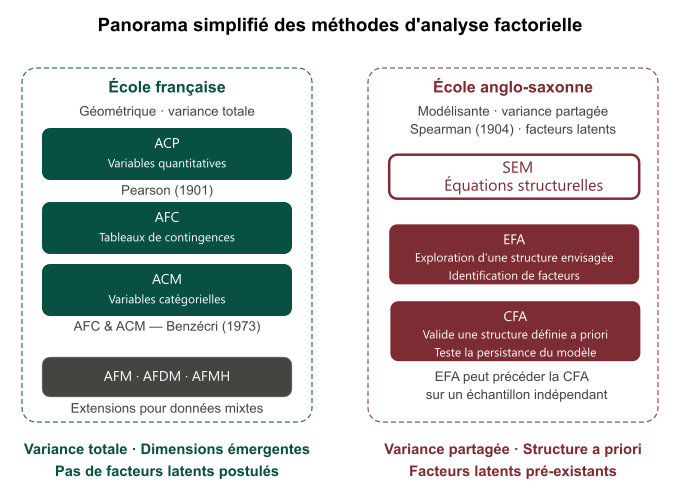
\includegraphics[keepaspectratio]{figures/panorama_af_def.png}}
\end{center}

Derrière ces deux écoles il y a des postures, des hypothèses fortes et
différentes. Outre la question de la variance et des facteurs latents
rapidement évoquée précédemment, et qui sera développée au point 2, il y
a une différence fondamentale de posture épistemique et donc d'hypothèse
de départ.

Dans le cadre de l'analyse \emph{à la française}, l'approche est
inductive, il s'agit de décrire, d'explorer des relations et des
distances. Pour Benzécri : \emph{``le modèle doit suivre les données,
non l'inverse''} (Jean-Paul Benzecri, L'Analyse des données. 2 :
L'analyse des correspondances, Paris, Bordas, 1973, p.~6.). Il n'y a
donc pas de modèle théorique préalable qui puisse être validé par ces
analyses. L'objectif est exploratoire. Il n'a pas de distribution
supposée, pas de facteurs pré-existants postulés.

En revanche, le socle de l'analyse factorielle \emph{à l'anglo-saxone}
est basé sur la confrontation d'un modèle théorique aux données. Le
postulat de départ repose sur l'existence de facteurs latents
pré-existant. C'est l'hypothèse fondatrice et la plus forte : les
variables observées sont causées par des construits sous-jacents non
mesurables directement (les facteurs latents). Les facteurs ne sont pas
construits par l'analyse, ils lui pré-existent et portent une part
explicative de la structuration des données obtenue. Le chercheur doit
avoir une théorie \emph{a priori} afin de mener de telles analyses. Il
s'agit d'une posture hypothético-déductive.

Si l'ACP et les méthodes popularisées par Benzécri ont su rester à la
postérité et servir dans toutes les SHS, notamment grâce à la mise en
oeuvre des méthodes pour travailler sur des données qualitatives, il
peut être utile de se rappeler qu'il en existe d'autres. Les méthodes
relevant de l'école anglo-saxonne, si elles sont très utilisées en
psychologie - discipline de Spearman, restent plus rares dans les autres
sciences humaines et sociales.

Dans cet article nous centrerons notre présentation sur les méthodes
d'analyses factorielles développées dans le contexte anglo-saxon.
Contrairement aux analyses factorielles de l'école française qui sont
employées dans un objectif exploratoire, ces méthodes de l'école
anglaise ont une approche modélisante, comme exposé précédemment.

Nous présenterons deux types d'analyses qui peuvent être réalisées
indépendamment mais qui sont souvent présentées successivement. Dans un
premier temps nous présenterons l'analyse factorielle exploratoire
(EFA), qui comme son nom ne l'indique pas n'est pas réalisée dans une
approche totalement exploratoire, car sa mise en oeuvre implique des
hypothèses précises que l'analyse testera. Puis dans un second temps
nous présenterons l'analyse factorielle confirmatoire (CFA), qui permet
de tester la persistance d'une structuration des données en éprouvant un
modèle pré-défini soit par une analyse exploratoire réalisée dans une
étape préalable, soit par ces deux types d'analyses factorielles
exploratoires et confirmatoires réalisées par d'autres auteurs. En
effet, la particularité de ce type d'analyse est la recherche de la
persistance d'une structuration de données alors modélisée. Très
utilisées en Psychologie pour le développement et l'utilisation d'outils
psychométriques (sous forme de questionnaire), les professionnels de
santé vont pouvoir reprendre des outils développés par d'autres sans
courir le risque qu'ils fonctionnent différemment. Il est donc essentiel
pour les chercheurs de s'assurer de la stabilité de ces outils avant de
les diffuser. Par exemple, afin de déterminer si un patient est déprimé
ou non, les professionnels de santé vont utiliser un outil
psychométrique dédié. Il n'est pas envisageable que cet outil détermine
à tort qu'une personne n'ait pas besoin de suivi psychologique parce que
l'outil aurait été mal conçu.

\section{Les méthodes anglaises d'Analyses Factorielles pour quoi faire
?}\label{les-muxe9thodes-anglaises-danalyses-factorielles-pour-quoi-faire}

Ces méthodes visent à explorer (dans le cadre d'une EFA) ou à valider
(dans le cadre d'une CFA) la structure sous-jacente d'une base de donnée
en identifiant des facteurs latents qui vont expliquer les relations
entre les variables de cette base de données.

Qu'est-ce qu'un facteur latent ? C'est une variable qui est
sous-jacente, car non observée ou mesurée directement. Ce facteur
sous-jacent est postulé pour expliquer les covariances (ou corrélations)
entre l'ensemble des variables observées, sélectionnées au préalable
dans le cadre d'hypothèses théoriques. Les variables observées, sont
mesurées directement, tandis que les facteurs latents ne le sont pas.

Cette notion de facteur latent est au coeur de ces méthodes d'analyses
factorielles. En effet l'idée centrale de ces méthodes est que les
variables mesurées sont influencées par ces facteurs latents, et que ces
facteurs vont expliquer la structure des relations des variables entre
elles. Chaque facteur latent est associé à un groupe de variables qui
partagent une variance commune. En d'autres termes, le facteur latent
exprime l'information partagée par un ensemble de variables.

Supposons que nous avons une base de données constituée de variables
mesurant un ensemble de critères observables. Par exemple, lors d'un
match de rugby nous avons collecté le nombre de mètres parcourus, de
points marqués, du nombre de passes, de plaquages\ldots{} On pourrait
postuler l'existance de facteurs latents qu'on pourrait appeler
\emph{performance} et \emph{vision de jeu}. Ces deux facteurs latents ne
peuvent pas être mesurés directement, mais peuvent être postulés pour
tenter d'expliquer la variation commune des variables observées/mesurées
qui rendent compte de ces deux facteurs latents.

Notre objectif lors de la réalisation d'une EFA sera d'identifier le
nombre et la nature de ces facteurs latents et de comprendre comment ils
sont associés et reliés aux variables mesurées. Cette méthode va donc
permettre de faire émerger un pattern de relations entre ces variables.
La structuration des facteurs obtenus ne sera peut-être pas exactement
celle envisagée au départ, mais l'EFA, bien que mentionnée comme
exploratoire, nécessite d'avoir des hypothèses concernant l'existance
des facteurs latents précisément testés. Par la suite une CFA pourra
être envisagée afin de vérifier si la structure obtenue avec l'EFA est
retrouvée auprès d'un autre échantillon d'une même population.

Ainsi, si l'objectif est d'explorer et d'identifier des dimensions
explicatives sous-jacentes, qui influencent des variables observées,
comme c'est souvent le cas en SHS, les analyses factorielles de l'école
anglo-saxonne s'avéreront être un bon choix.

\subsection{ACP et FA, quelles différences
?}\label{acp-et-fa-quelles-diffuxe9rences}

Les différences entre ces deux familles de méthodes sont donc
importantes. Elles ne sont pas seulement épistémiques mais aussi
statistiques et pas toujours si simples à appréhender intuitivement.
Nous l'avons évoqué, ces méthodes vont différer tant dans leur objectif
que dans leur approche. Voici trois nouveaux points de divergence, qu'il
est nécessaire de prendre en compte pour faire un choix éclairé entre
\textbf{Analyse en Composantes Principales} et \textbf{Analyse
Factorielle} : l'objectif statistique principal, la nature des variables
et l'interprétation des résultats.

1- L'objectif statistique principal :

ACP et FA ont comme objectif commun la réduction de l'information, mais
elles ne vont pas du tout opérer de la même manière.

\begin{itemize}
\tightlist
\item
  Les ACP : l'objectif est de réduire la dimensionnalité des données en
  utilisant les composantes principales. L'ACP va transformer les
  variables observées en un ensemble de variables non corrélées, que
  l'on appelle composantes principales, qui ne pré-existaient pas à
  l'analyse contrairement aux facteurs latents. La composante principale
  est une combinaison linéaire des variables originales qui prend en
  compte la part de variance la plus élevée présente dans les données.
  Ces composantes principales sont classées par ordre décroissant de
  l'importance de la variance qu'elles capturent. Tout l'enjeu de l'ACP
  est de définir des composantes principales qui permettent de réduire
  la dimensionnalité des données tout en conservant l'information
  essentielle contenue dans les variables d'origine. Les composantes
  principales étant des variables non corrélées entre elles, cela
  simplifie l'interprétation des relations entre les observations.
  \emph{Pour résumer, l'objectif principal de l'ACP est de synthétiser
  les données en composantes principales en tentant de conserver le
  maximum de variance des variables de la base de données.}
\item
  Les FA : visent à explorer la structure sous-jacente des données en
  identifiant des facteurs latents qui expliquent les relations entre
  les variables observées. L'objectif est de réduire la dimensionnalité
  des données en se centrant sur la variance partagée entre les
  variables et non sur l'ensemble des données. Dans le cadre de l'EFA,
  une partie de la variance des données ne sera pas retenue dans le
  modèle. L'objectif n'étant pas de conserver le maximum de variance de
  l'ensemble de données, mais bien de se centrer sur la variance
  partagée entre les différentes variables. Ces analyses sont
  généralement réalisées sur les variables d'un ensemble de données,
  contrairement aux analyses en composantes principales qui peuvent être
  effectuées aussi bien sur des variables que sur des observations.
\end{itemize}

2- La nature des variables :

\begin{itemize}
\tightlist
\item
  Les ACP : Les variables de la base de données sont considérées comme
  des mesures directes. On cherche à réduire la dimensionnalité sans
  nécessairement interpréter les composantes principales en tant que
  telles.
\item
  Les FA : Les variables sont considérées comme des indicateurs de
  facteurs latents. On souhaite comprendre la structure sous-jacente de
  la base de données.
\end{itemize}

3- Interprétabilité :

\begin{itemize}
\tightlist
\item
  Les ACP : Les composantes principales sont des combinaisons linéaires
  des variables originales et peuvent être peu interprétables du point
  de vue conceptuel. On va considérer le poids ou la contribution d'une
  variable pour chaque composante principale, ce qui va permettre de
  mesurer l'importance relative des variables dans la variance totale
  des données.
\item
  Les FA : Les facteurs latents identifiés s'interprètent comme des
  concepts sous-jacents aux données, mais qu'il est nécessaire
  d'identifier et de théoriser. Ce travail doit être fait en amont de la
  réalisation des analyses. L'interprétation, repose sur l'étude des
  charges factorielles associées à chaque facteur latent. Il s'agit tout
  simplement des corrélations de chaque variable avec chaque facteur
  latent. Ces corrélations permettent d'étudier la relation entre les
  variables et les facteurs latents, et donc de donner du sens à ces
  facteurs alors identifiés.
\end{itemize}

Le choix entre ces deux familles de méthodes repose globalement sur ce
que l'on veut étudier et de ce que l'on veut faire de la variance. Si on
considère qu'il n'y a pas de facteur latent et que l'on souhaite
conserver le maximum de la variance des données alors les méthodes de la
famille des ACP est un choix tout à fait pertinent. En revanche, si on
envisage une structure sous-jacente à nos données, et donc la présence
de facteurs latents, et que l'on estime qu'il n'est pas forcément
nécessaire de conserver toute la variance de nos données, mais
uniquement celle qui est partagée entre nos variables, alors les FA
seront le bon choix.

\subsection{Limites des FA}\label{limites-des-fa}

Comme toutes les méthodes d'analyse de données les FA comportent des
limites.

\textbf{Le type de variable}

La limite majeure des FA, repose sur le fait que cette méthode est plus
efficiente avec des variables continues. Toutefois, il est tout-à-fait
possible de l'utiliser avec des variables ordonnées : catégories qui
suivent un ordre, (par ex. de \emph{1. ``Pas du tout d'accord''} à
\emph{5. ``Tout-à-fait d'accord''}) en traduisant chaque catégorie par
un score. On peut également réaliser ce type d'analyse avec des
variables catégorielles (catégories sans échelle de valeur entre elles
par ex. : profession), mais il faudra alors être beaucoup plus prudent
sur l'interprétation. Et selon les cas, il peut être plus pertinent
d'utiliser une autre méthode de factorisation comme l'analyse
factorielle des correspondances (AFC) ou une analyse des correspondances
multiples (ACM).

\textbf{La taille de l'échantillon}

La taille de l'échantillon est également un élément contraignant pour ce
type d'analyse. Si l'échantillon est trop faible au regard de la taille
des informations à synthétiser, les résultats obtenus risquent de
surreprésenter les spécificités de la population alors testée. La
structure de l'analyse ne sera pas généralisable, mais influencée par
les spécificités de l'échantillon. Il est donc important d'avoir une
taille d'échantillon suffisamment importante afin de pallier ce type de
biais (Young and Pearce 2013). L'échantillon devra être sélectionné
selon le nombre de variables contenues dans l'analyse et la force du
lien entre les variables mesurées et les facteurs latents (Watkins, M.
W., 2018). Plus ce lien sera fort, moins il sera nécessaire d'avoir un
échantillon conséquent. Certains auteurs indiquent que si les
corrélations entre les variables manifestes et les facteurs latents sont
plutôt fortes (aux alentours de 0.80), 150 observations peuvent suffire
à réaliser une méthode qui relève des FA. En revanche, si ces mêmes
corrélations sont plutôt faibles (inférieures à 0.40) il serait alors
nécessaire d'avoir un échantillon d'au-moins 300 observations pour
retrouver une structure factorielle stable (Schreiber, J., 2021).

\textbf{La force des liens}

Des corrélations trop fortes ou trop faibles entre les variables peuvent
mettre en péril la mise en facteur des informations, mais pas pour les
mêmes raisons. Si l'ensemble de variables soumis à la factorisation
n'est pas du tout corrélé, alors les éléments présentés ne partagent pas
d'éléments communs et ne peuvent pas être résumés sous un même facteur.
L'hétérogénéité des informations peut tout-à-fait empêcher son résumé
statistique via l'utilisation des analyses factorielles. Il n'est pas
possible de réaliser des analyses factorielles sur des ensembles de
variables non-corrélées. A l'inverse, si les variables retenues pour
l'analyse sont trop fortement corrélées alors ceci sous-tend qu'elles
contiennent des informations tellement similaires qu'elles en sont
redondantes. Cette redondance peut tout-à-fait biaiser la factorisation
des informations, car certains éléments seront surreprésentés - sans que
cela ne reflète une quelconque réalité - par rapport à d'autres. Ce
problème peut être résolu en sélectionnant uniquement l'une des deux
variables représentatives d'un même phénomène. Par exemple, la catégorie
socio-professionnelle et le niveau de diplôme sont généralement très
corrélés, il faudra sélectionner l'une de ces deux variables dans le
modèle d'analyse factorielle pour que celui-ci soit optimal (Tabachnick,
B., \& Fidell, L., 2014).

\textbf{L'interprétation}

La subjectivité de l'interprétation peut aussi être une limite,
notamment sur l'identification et l'interprétation des facteurs latents,
qui dépendra beaucoup du chercheur et de son positionnement théorique.

\subsection{Les FA aujourd'hui en sciences
humaines}\label{les-fa-aujourdhui-en-sciences-humaines}

En SHS aujourd'hui les FA sont surtout utilisées en psychologie, et ce
depuis de nombreuses années. La validation des tests psychométriques
constitue un exemple classique de l'utilisation de l'EFA et de son
utilisation conjointe avec l'Analyse factorielle confirmatoire (CFA), à
l'image de l'association régulièrement employée entre ACP et CAH
(Classification Ascendante Hiérarchique) pour classer des observations.
L'analyse factorielle exploratoire et confirmatoire se complètent
également très bien. Il est d'ailleurs très fréquent que ces deux
méthodes soient utilisées ensemble. C'est même plutôt recommandé, tels
que l'argumentent Flora \& Flake dans un article paru en 2017 (Flora \&
Flake, 2017). Afin de réaliser des tests standardisés pour évaluer des
processus psychologiques, les psychologues ont recours à ce couple
d'analyses factorielles, en réalisant une analyse factorielle
exploratoire sur un premier échantillon et une analyse factorielle
confirmatoire sur un second échantillon (ayant tous 2 les mêmes
caractéristiques). Il est donc nécessaire d'avoir une base de données
avec un grand nombre d'observations afin de permettre la création d'un
échantillon d'entrainement et de test suffisamment grands. Réaliser ces
analyses exploratoires et confirmatoires sur deux échantillons
différents permet d'éliminer toute spécificité liée à l'échantillonnage.

Les psychologues se sont tournés vers ces techniques de réduction des
dimensions car, pour la plupart de leurs études, ils souhaitent se
centrer sur la variance partagée entre chaque item, plutôt que de
chercher à conserver la variance totale d'un ensemble de variables. Le
processus méthodologique alors suivi permet de faire émerger une
structure factorielle sans nécessairement la totalité des variables
présentes. Cette structure factorielle permet d'observer comment les
variables du jeu de données rendent compte des facteurs latents qui les
sous-tendent. L'objectif finalement est de savoir \emph{``Est-ce que je
mesure bien ce que je pense mesurer ?''}. En d'autres termes, est-ce que
les questions posées aux répondants sont adaptées pour accéder à une
dimension latente non appréhendable directement.

Un point important nous semble à présent à souligner, sur l'utilisation
des analyses factorielles exploratoires et confirmatoires. A partir du
moment où un test psychométrique (en Psychologie) ou un questionnaire
est validé, c'est-à-dire qu'il a déjà été éprouvé par le couple EFA/CFA
sur un jeu de données assez conséquent, avec une population ayant les
mêmes caractéristiques, il n'est pas nécessaire de remettre en cause la
structure du test. Nous pouvons directement procéder à une analyse
factorielle confirmatoire (CFA), afin de vérifier si le modèle, alors
pré-établi par d'autres, s'ajuste à nos données. Ceci est conseillé afin
de ne pas multiplier les tests statistiques et entraîner une inflation
des résultats faussement positifs (encore appelés erreur de type I). Dit
plus simplement cela permet d'avoir un étalonnage et de pouvoir comparer
les populations vis-à-vis d'un même outil. Les psychologues ont des
outils étalonnés pour mesurer les croyances dans les phénomènes
paranormaux par exemple. On pourrait très bien imaginer que les sciences
sociales procèdent de la même manière sur d'autres thématiques afin de
soumettre le même questionnaire à différents échantillons d'une même
population.

Cette approche statistique, très courante en psychologie, peut
tout-à-fait être appliquée aux autres disciplines des SHS, à la fois sur
l'exploration des bases de données (EFA), ou sur une comparaison dans le
temps (couple EFA/CFA). Nous verrons dans cet article comment adapter ce
processus statistique à des données non psychologiques.

\section{Les packages}\label{les-packages}

\begin{Shaded}
\begin{Highlighting}[]
\ControlFlowTok{if}\NormalTok{ (}\SpecialCharTok{!}\FunctionTok{require}\NormalTok{(}\StringTok{"pacman"}\NormalTok{)) }\FunctionTok{install.packages}\NormalTok{(}\StringTok{"pacman"}\NormalTok{)}
\NormalTok{pacman}\SpecialCharTok{::}\FunctionTok{p\_load}\NormalTok{(correlation, corrplot, dplyr, EFA.dimensions, effectsize, ggraph, ggplot2, here, lavaan, nFactors, parallel, parameters, psych, rrcov, RColorBrewer, see, semPlot, SemTools, table1, usdm)}
\end{Highlighting}
\end{Shaded}

A quoi servent ces différents packages ?

Les packges spécifiques aux méthodes d'Analyse Factorielle présentées :

\begin{itemize}
\item
  Les packages
  \emph{\href{https://cran.r-project.org/web/packages/EFA.dimensions/index.html}{EFA.dimensions}},
  \emph{\href{https://cran.r-project.org/web/packages/nFactors/index.html}{nfactors}},
  \emph{\href{https://cran.r-project.org/web/packages/psych/index.html}{psych}}
  et
  \emph{\href{https://stat.ethz.ch/R-manual/R-devel/library/parallel/doc/parallel.pdf}{parallel}}
  sont des packages utilisés pour vérifier si les données sont
  factorisables grâce à différents indices statistiques (KMO, etc.). Ils
  permettent également de déterminer le nombre de facteurs optimal à
  retenir selon l'ensemble de données soumis à l'analyse.
\item
  Le package \emph{\href{https://lavaan.ugent.be/}{lavaan}} permet de
  réaliser des modèles statistiques impliquant des variables latentes,
  telles qu'elles existent dans les Analyses factorielles exploratoires
  et confirmatoires.
\item
  Le package
  \emph{\href{https://cran.r-project.org/web/packages/effectsize/index.html}{effectsize}}
  pour interpréter les coefficients de l'analyse factorielle
  confirmatoire
\item
  Les packages
  \emph{\href{https://cran.r-project.org/web/packages/semPlot/index.html}{semPlot}}
  et
  \emph{\href{https://cran.r-project.org/web/packages/semTools/index.html}{semTools}}
  pour réaliser des equations structurelles méthode à laquelle
  appartient l'analyse factorielle confirmatoire
\end{itemize}

Les packages non-spécifiques aux méthodes présentées :

\begin{itemize}
\item
  \emph{\href{https://cran.r-project.org/web/packages/pacman/index.html}{pacman}}
  : est un package de management de packages.
\item
  \emph{\href{https://cran.r-project.org/web/packages/here/index.html}{here}}
  : permet de gérer les chemin d'accès au sein de notre projet
\item
  \emph{\href{https://cran.r-project.org/web/packages/dplyr/index.html}{dplyr}}
  est un package de manipulation de données.
\item
  Les packages
  \emph{\href{https://cran.r-project.org/web/packages/parameters/index.html}{parameters}},
  et
  \emph{\href{https://cran.r-project.org/web/packages/table1/vignettes/table1-examples.html}{table1}}
  sont utilisés dans cette fiche pour réaliser des statistiques
  descriptives et des mises en forme de sortie exploitables directement.
\item
  les packages
  \emph{\href{https://cran.r-project.org/web/packages/correlation/index.html}{correlation}}
  et
  \emph{\href{https://cran.r-project.org/web/packages/corrplot/vignettes/corrplot-intro.html}{corrplot}}
  permettent de réaliser des corrélations et des graphiques tels que des
  corrélogrammes.
\item
  Le package
  \emph{\href{https://cran.r-project.org/web/packages/usdm/usdm.pdf}{usdm}}
  comprend différentes fonctions permettant d'explorer l'impact de
  différentes sources d'incertitudes dans des mesures d'association.
  Nous utiliserons surtout les fonctions permettant de mesurer la
  multicolinéarité entre des variables.
\item
  \emph{\href{https://cran.r-project.org/web/packages/ggraph/index.html}{ggraph}},
  \emph{\href{https://cran.r-project.org/web/packages/ggplot2/index.html}{ggplot2}},
  \emph{\href{https://cran.r-project.org/web/packages/RColorBrewer/index.html}{RColorBrewer}}
  et
  \emph{\href{https://cran.r-project.org/web/packages/see/index.html}{see}}
  sont des packages dédiés à la production de représentations
  graphiques.
\end{itemize}

\section{Les données}\label{les-donnuxe9es}

L'idée de cet article est de présenter des méthodes d'analyse
factorielle issues de l'école anglo-saxonne et de voir comment elles
peuvent constituer une alternative aux analyses en composantes
principales.

Pour illustrer l'intérêt de ces méthodes en dehors de la psychologie,
nous utiliserons des données issues de travaux en géographie. Ces
dernières portent sur le prix de l'immobilier. La dimension spatiale de
ces données ne sera pas exploitée, ce n'est pas l'objectif des analyses
factorielles.

Les données du prix de l'immobilier par EPCI (prix médian au m²) sont
issues des ventes observées sur l'année 2018, extraites depuis la base
de données des notaires de France par Frédéric Audard et Alice Ferrari.
Ce fichier a été simplifié pour ne conserver que les variables d'intérêt
parmi une cinquantaine Les données statistiques proviennent de l'INSEE
(année 2019) : 9 variables ont été choisies pour leur potentialité à
expliquer les variations des prix de l'immobilier, concernant la
population, le logement et les revenus et niveaux de vie.

Ce fichier est composé des 9 variables suivantes :

\begin{itemize}
\tightlist
\item
  \emph{prix\_med} : prix médian par EPCI à la vente au m²
\item
  \emph{perc\_log\_vac} : \% logements vacants
\item
  \emph{perc\_maison} : \% maisons
\item
  \emph{perc\_tiny\_log} : \% petits logements
\item
  \emph{dens\_pop} : densité de population
\item
  \emph{med\_niveau\_vis} : médiane du niveau de vie
\item
  \emph{part\_log\_suroccup} : \% logements suroccupés
\item
  \emph{part\_agri\_nb\_emploi} : \% agriculteurs
\item
  \emph{part\_cadre\_profintellec\_nbemploi} : \% cadres et professions
  intellectuelles
\end{itemize}

Afin de réaliser le couple d'analyse EFA/CFA, comme expliqué
précédemment, nous devons partitionner les données en 2 ensembles
distincts. Cette partition est réalisée de façon aléatoire entre les
observations. Nous obtiendrons deux ensembles de données, l'un pour
réaliser l'EFA et l'autre pour effectuer la CFA.

\href{https://github.com/LeCampionG/Article_Rzine-AFE/raw/main/data/data.zip}{{}
Télécharger les données}

\begin{Shaded}
\begin{Highlighting}[]
\CommentTok{\# Chargement des données de base}

\FunctionTok{library}\NormalTok{(here)}
\NormalTok{csv\_path }\OtherTok{\textless{}{-}} \FunctionTok{here}\NormalTok{(}\StringTok{"data"}\NormalTok{, }\StringTok{"immo\_afe.csv"}\NormalTok{)}

\NormalTok{dfz}\OtherTok{\textless{}{-}} \FunctionTok{read.csv2}\NormalTok{(csv\_path, }\AttributeTok{row.names=}\DecValTok{1}\NormalTok{)}
\end{Highlighting}
\end{Shaded}

\textbf{Partitionnement des données :}

\begin{Shaded}
\begin{Highlighting}[]
\DocumentationTok{\#\# Indiquer une graine pour conserver la même répartition lors des partitionnements à chaque exécution du script}
\FunctionTok{set.seed}\NormalTok{(}\DecValTok{345}\NormalTok{)}
\DocumentationTok{\#\# En premier lien le partitionnement des data}
\NormalTok{partitions }\OtherTok{\textless{}{-}}\NormalTok{ datawizard}\SpecialCharTok{::}\FunctionTok{data\_partition}\NormalTok{(dfz, }\AttributeTok{proportion =} \FloatTok{0.5}\NormalTok{) }\CommentTok{\# ici division du corpus eavec 50\% des individus dasn l\textquotesingle{}échantillon d\textquotesingle{}entrainement}
\NormalTok{training }\OtherTok{\textless{}{-}}\NormalTok{ partitions}\SpecialCharTok{$}\NormalTok{p\_0}\FloatTok{.5}
\NormalTok{test }\OtherTok{\textless{}{-}}\NormalTok{ partitions}\SpecialCharTok{$}\NormalTok{test}

\NormalTok{training}\SpecialCharTok{$}\NormalTok{.row\_id }\OtherTok{\textless{}{-}} \ConstantTok{NULL}
\NormalTok{test}\SpecialCharTok{$}\NormalTok{.row\_id }\OtherTok{\textless{}{-}} \ConstantTok{NULL}
\end{Highlighting}
\end{Shaded}

Nous obtenons deux ensembles de données, l'un comprenant 612
observations, sur lequel nous réaliserons l'EFA, et le second comptant
611 observations sur lequel nous réaliserons la CFA.

\section{Mise en pratique : exemple du prix de l'immobilier en France
hexagonale}\label{mise-en-pratique-exemple-du-prix-de-limmobilier-en-france-hexagonale}

Il est extrêmement recommandé de centrer-réduire ses données pour
réaliser une analyse statistique multivariée telle qu'une analyse
factorielle, ou plus généralement lorsque l'on travaille avec des
variables n'étant pas sur les mêmes échelles, sur les mêmes ordres de
grandeurs. Cela implique de faire subir aux données une transformation
statistique visant à ce qu'elles aient une moyenne de 0 et un écart-type
de 1. On parle aussi en statistique de standardisation. Cette
transformation permet de conserver la variabilité des données (la
distance entre chaque valeur reste inchangée), tout en les rendant
comparables (elles sont placées sur une même échelle). Dans le cadre de
modélisations statistiques, il est nécessaire de réaliser cette
opération sur les variables explicatives du modèle. Sur R, cette
opération peut se réaliser facilement avec la fonction \texttt{scale()}
- que nous utilisons dans l'exemple présenté - ou à ``la main''.
L'opération est simple : il s'agit de soustraire chaque valeur par la
moyenne puis de divise chaque valeur par l'écart-type. Dans notre
exemple cette opération a déjà été effectuée précédemment. Les données
chargées sont donc déjà centrées et réduites.

La première étape étant toujours la description des données, voici le
code pour réaliser un tableau récapitulatif des variables, ici sur le
prix de l'immobilier. Dans cette partie, nous ne présentons les
statistiques descriptives que sur l'une des deux bases de données
(\emph{training}) pour plus de lisibilité. Néanmoins, nous avons bien
vérifié les statistiques descriptives sur les deux ensembles de données.

\begin{Shaded}
\begin{Highlighting}[]
\FunctionTok{table1}\NormalTok{(}\SpecialCharTok{\textasciitilde{}}\NormalTok{ prix\_med }\SpecialCharTok{+}\NormalTok{ perc\_log\_vac }\SpecialCharTok{+}\NormalTok{ perc\_maison }\SpecialCharTok{+}\NormalTok{ perc\_tiny\_log }\SpecialCharTok{+}\NormalTok{ dens\_pop }\SpecialCharTok{+}\NormalTok{ med\_niveau\_vis }\SpecialCharTok{+}\NormalTok{ part\_log\_suroccup }\SpecialCharTok{+}\NormalTok{ part\_agri\_nb\_emploi }\SpecialCharTok{+}\NormalTok{ part\_cadre\_profintellec\_nbemploi , }\AttributeTok{data=}\NormalTok{training) }
\end{Highlighting}
\end{Shaded}

La réalisation des représentations graphiques permet d'appréhender les
distributions des variables et leurs éventuelles spécificités. Voici une
façon de réaliser un diagramme des distributions des variables.

\begin{Shaded}
\begin{Highlighting}[]
\CommentTok{\#| results: \textquotesingle{}hide\textquotesingle{}}
\CommentTok{\#| fig{-}width: 9}
\CommentTok{\#| fig{-}height: 9}


\NormalTok{dfgraph}\OtherTok{\textless{}{-}}\FunctionTok{subset}\NormalTok{(training, }\AttributeTok{select =} \FunctionTok{c}\NormalTok{(prix\_med, perc\_log\_vac, perc\_maison, perc\_tiny\_log, dens\_pop, med\_niveau\_vis, part\_log\_suroccup, part\_agri\_nb\_emploi, part\_cadre\_profintellec\_nbemploi))}

\NormalTok{op }\OtherTok{\textless{}{-}} \FunctionTok{par}\NormalTok{(}\AttributeTok{mfrow =} \FunctionTok{c}\NormalTok{(}\DecValTok{3}\NormalTok{, }\DecValTok{3}\NormalTok{), }\AttributeTok{mar =} \FunctionTok{c}\NormalTok{(}\DecValTok{3}\NormalTok{, }\DecValTok{3}\NormalTok{, }\FloatTok{1.5}\NormalTok{, }\DecValTok{1}\NormalTok{))  }\CommentTok{\# marges réduites}

\NormalTok{h1 }\OtherTok{\textless{}{-}} \FunctionTok{hist}\NormalTok{(dfgraph}\SpecialCharTok{$}\NormalTok{prix\_med, }\AttributeTok{main=}\ConstantTok{NULL}\NormalTok{)}
\NormalTok{h2 }\OtherTok{\textless{}{-}} \FunctionTok{hist}\NormalTok{(dfgraph}\SpecialCharTok{$}\NormalTok{perc\_log\_vac, }\AttributeTok{main=}\ConstantTok{NULL}\NormalTok{)}
\NormalTok{h3 }\OtherTok{\textless{}{-}} \FunctionTok{hist}\NormalTok{(dfgraph}\SpecialCharTok{$}\NormalTok{perc\_maison, }\AttributeTok{main=}\ConstantTok{NULL}\NormalTok{)}
\NormalTok{h4 }\OtherTok{\textless{}{-}} \FunctionTok{hist}\NormalTok{(dfgraph}\SpecialCharTok{$}\NormalTok{perc\_tiny\_log, }\AttributeTok{main=}\ConstantTok{NULL}\NormalTok{)}
\NormalTok{h5 }\OtherTok{\textless{}{-}} \FunctionTok{hist}\NormalTok{(dfgraph}\SpecialCharTok{$}\NormalTok{dens\_pop, }\AttributeTok{main=}\ConstantTok{NULL}\NormalTok{)}
\NormalTok{h6 }\OtherTok{\textless{}{-}} \FunctionTok{hist}\NormalTok{(dfgraph}\SpecialCharTok{$}\NormalTok{med\_niveau\_vis, }\AttributeTok{main=}\ConstantTok{NULL}\NormalTok{)}
\NormalTok{h7 }\OtherTok{\textless{}{-}} \FunctionTok{hist}\NormalTok{(dfgraph}\SpecialCharTok{$}\NormalTok{part\_log\_suroccup, }\AttributeTok{main=}\ConstantTok{NULL}\NormalTok{)}
\NormalTok{h8 }\OtherTok{\textless{}{-}} \FunctionTok{hist}\NormalTok{(dfgraph}\SpecialCharTok{$}\NormalTok{part\_agri\_nb\_emploi, }\AttributeTok{main=}\ConstantTok{NULL}\NormalTok{)}
\NormalTok{h9 }\OtherTok{\textless{}{-}} \FunctionTok{hist}\NormalTok{(dfgraph}\SpecialCharTok{$}\NormalTok{part\_cadre\_profintellec\_nbemploi, }\AttributeTok{main=}\ConstantTok{NULL}\NormalTok{)}
\end{Highlighting}
\end{Shaded}

\pandocbounded{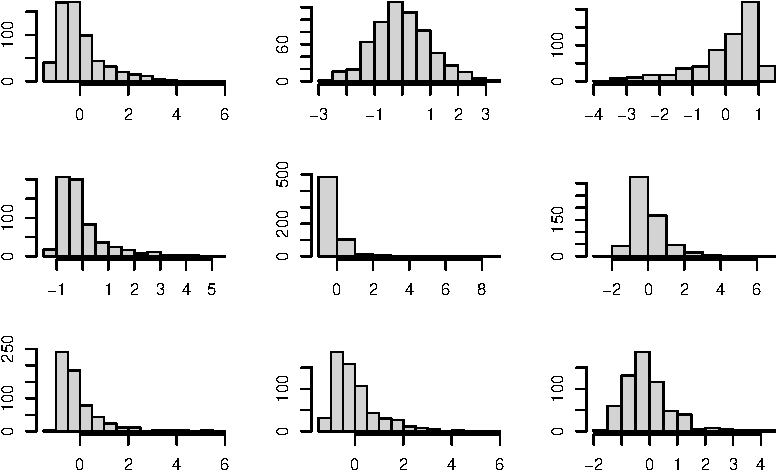
\includegraphics[keepaspectratio]{index_files/figure-pdf/unnamed-chunk-5-1.pdf}}

\begin{Shaded}
\begin{Highlighting}[]
\FunctionTok{par}\NormalTok{(op)  }\CommentTok{\# restaure marge}
\end{Highlighting}
\end{Shaded}

\subsection{Les pré-requis de l'analyse
factorielle}\label{les-pruxe9-requis-de-lanalyse-factorielle}

Comme toutes les méthodes statistiques les analyses factorielles ont un
certain nombre de pré-requis à vérifier. Ne pas en tenir compte nous
expose à des résultats biaisés voire complètement erronés.

\subsubsection{Les Outliers : comment les gérer
?}\label{les-outliers-comment-les-guxe9rer}

La question du traitement de ces individus extrêmes est loin d'être
simple. Elle doit faire l'objet d'une réflexion et de choix importants
qu'il faut pouvoir assumer tant statistiquement que théoriquement.

Les outliers sont les individus extrêmes. Il est toujours nécessaire de
pouvoir les identifier afin de savoir comment les gérer. L'enjeu autour
de ces individus c'est qu'ils vont nécessairement influencer (voire
fausser) les résultats des analyses. Les résultats obtenus pourront être
différents s'ils sont conservés ou retirés de l'analyse (Zijlstra et
al.~2011). Si les résultats diffèrent il sera nécessaire de les
présenter avec et sans les individus extrêmes, ainsi que d'expliciter la
conclusion retenue pour plus de transparence.

Il existe un grand nombre d'indicateurs et de distances qui permettent
d'identifier des outliers. Nous ne les présenterons pas dans le cadre de
cet article. Il existe différents travaux sur le sujet pouvant vous
éclairer, dont voici un aperçu (Aguinis et al.~2013 ; Bakker, M., \&
Wicherts, J. M., 2014 ; Leys et al.~2018 ; Leys et al.~2019, etc.).

Nous testons donc la présence d'individus extrêmes sur les deux bases de
données \emph{training} et \emph{test}.

Pour la base de données \emph{training}, voici le code. Nous utilisons
la distance de MCD robuste, qui est conseillée par la littérature dans
un contexte d'analyse multivariée.

D'après nos connaissances il n'existe pas de seuils précis afin de
déterminer si une observation extrême doit être supprimée ou non avec la
méthode MCD robuste. En effet, il n'existe pas de règles pré-établies en
la matière. Nous choisissons donc de supprimer les observations que nous
considérons très éloignées du reste de l'échantillon à la lecture
graphique. Nous avons supprimé 25 observations pour cette première base
de données \emph{training}. Après cette suppression, nous avons vérifié
à nouveau la présence d'observations extrêmes. Cette nouvelle lecture
graphique ne témoignant pas d'un éloignement visible important, nous
avons décidé de ne pas supprimer davantage d'observations.

Nous avons supprimé 18 observations pour cette seconde base de données,
\emph{test}. Après cette suppression, nous avons vérifié à nouveau la
présence d'observations extrêmes. Cette nouvelle lecture graphique ne
témoignant pas d'un éloignement visible important, nous avons décidé de
ne pas supprimer davantage d'observations.

Nous avons retiré 43 outliers des bases de données sur le prix de
l'immobilier. C'est-à-dire que nous avons supprimé 43 EPCI ayant des
valeurs très éloignées des autres sur cet aspect. Parmi les EPCI
concernés, il y a notamment le grand Paris, mais également d'autres
localités où le prix de l'immobilier est particulièrement élevé, telle
que la communauté de communes d'Annemasse les Voirons, frontalière avec
la Suisse. Mais le prix de l'immobilier n'est pas le seul élément qui
caractérise les valeurs extrêmes identifiées, car notre analyse est
multivariée et tient en compte d'autres indicateurs tels que la part de
logements vacants ou encore le niveau de vie médian. Pour cet article
nous avons fait le choix de supprimer ces EPCI de notre analyse. En
effet, nous cherchons à mettre en évidence des facteurs latents,
s'exprimant au travers des variables mesurées, qui caractérisent les
EPCI de la France Hexagonale. Or malheureusement si nous conservons ces
valeurs extrêmes nous nous exposons à ne pas observer la variabilité des
différents EPCI de l'hexagone, mais uniquement de la distance entre ces
EPCI où le prix de l'immobilier est particulièrement élevé et les autres
EPCI de la base de données. Ces EPCI étant tellement éloignés des autres
EPCI sur l'ensemble des variables de la base de données que ceux-ci
écrasent les variabilités entre les autres communes. Afin de pouvoir
faire émerger une structure factorielle qui ait du sens entre les EPCI,
nous faisons le choix de sortir ces EPCI éloignés des autres de nos
analyses.

Les scripts des traitements des valeurs extrêmes sur les bases de
données \emph{training} et \emph{test} sont disponibles en annexe.

Les données sans valeurs extrêmes sont dans les bases \emph{trainingp}
et \emph{testp}.

\subsubsection{Analyse de la matrice de
corrélation}\label{analyse-de-la-matrice-de-corruxe9lation}

L'analyse des corrélations est une étape toujours essentielle dans
l'analyse de données, et notamment dans le cadre de la modélisation
statistique.

Cette étape est fondamentale pour plusieurs raisons. D'abord car elle
permet d'étudier les relations entre les variables, ce qui va donner des
indications sur le meilleur modèle pour les données sélectionnées. En
effet, des corrélations trop fortes ou à l'inverse une absence totale de
corrélation peut poser de nombreux problèmes comme nous l'avons évoqué
précédemment. Par exemple:

\begin{itemize}
\tightlist
\item
  \emph{La multi-colinéarité} : Lorsque des variables sont trop
  fortement corrélées (positivement ou négativement) cela pose un
  problème de multi-colinéarité. Les variables sont tellement liées
  qu'il devient difficile de distinguer leur impact individuel, cela va
  rendre les résultats peu fiables. Il deviendra compliqué d'interpréter
  les coefficients et de comprendre de quoi rend-il vraiment compte.
\item
  \emph{Des risques de surajustement} : Un modèle avec des prédicteurs
  trop fortement corrélés va être surajusté et donc ne sera pas
  pertinent dans son rôle prédictif.
\item
  \emph{Une instabilité du modèle} : Les modèles avec des variables trop
  fortement corrélées sont instables. La moindre variation dans les
  données pourra provoquer de très grandes variations dans les
  résultats.
\item
  \emph{Un modèle non optimisé} : Un modèle doit respecter le principe
  de parcimonie. Il ne faut pas qu'il contienne de variables redondantes
  (corrélations trop fortes) ou inutiles (absence de corrélations).
\item
  \emph{Un modèle nul} : Une absence totale de corrélations remet en
  question la pertinence de tester, dans un même modèle, des variables
  qui n'auraient donc aucun rapport entre elles.
\end{itemize}

Comme nous avons pu l'observer précédemment avec les histogrammes des
distributions des variables, celles-ci ne suivent pas une loi normale.
Le coefficient de corrélation de Pearson n'étant pas stable sur des
données non-normales, nous lui préfererons celui de Spearman pour
calculer la matrice de corrélation.

Pour plus de lisibilité nous ne présentons la matrice de corrélation que
sur la base \emph{trainingp}, mais celle-ci a également été réalisée sur
la base \emph{testp}.

\begin{Shaded}
\begin{Highlighting}[]
\CommentTok{\# Matrice de corrélation}
\NormalTok{cor }\OtherTok{\textless{}{-}} \FunctionTok{correlation}\NormalTok{(trainingp, }\AttributeTok{method =} \StringTok{"spearman"}\NormalTok{)}
\NormalTok{cor }\SpecialCharTok{\%\textgreater{}\%}
  \FunctionTok{summary}\NormalTok{(}\AttributeTok{redundant =} \ConstantTok{FALSE}\NormalTok{)}
\end{Highlighting}
\end{Shaded}

\begin{verbatim}
# Correlation Matrix (spearman-method)

Parameter           | part_cadre_profintellec_nbemploi | part_agri_nb_emploi
----------------------------------------------------------------------------
prix_med            |                          0.48*** |            -0.54***
perc_log_vac        |                         -0.32*** |             0.45***
perc_maison         |                         -0.52*** |             0.64***
perc_tiny_log       |                          0.64*** |            -0.63***
dens_pop            |                          0.67*** |            -0.78***
med_niveau_vis      |                          0.43*** |            -0.43***
part_log_suroccup   |                          0.45*** |            -0.53***
part_agri_nb_emploi |                         -0.68*** |                    

Parameter           | part_log_suroccup | med_niveau_vis | dens_pop
-------------------------------------------------------------------
prix_med            |           0.40*** |        0.66*** |  0.57***
perc_log_vac        |          -0.18*** |       -0.57*** | -0.46***
perc_maison         |          -0.68*** |       -0.24*** | -0.47***
perc_tiny_log       |           0.76*** |        0.22*** |  0.60***
dens_pop            |           0.36*** |        0.49*** |         
med_niveau_vis      |              0.04 |                |         
part_log_suroccup   |                   |                |         
part_agri_nb_emploi |                   |                |         

Parameter           | perc_tiny_log | perc_maison | perc_log_vac
----------------------------------------------------------------
prix_med            |       0.39*** |    -0.48*** |     -0.79***
perc_log_vac        |       -0.14** |     0.27*** |             
perc_maison         |      -0.68*** |             |             
perc_tiny_log       |               |             |             
dens_pop            |               |             |             
med_niveau_vis      |               |             |             
part_log_suroccup   |               |             |             
part_agri_nb_emploi |               |             |             

p-value adjustment method: Holm (1979)
\end{verbatim}

Les résultats sont similaires pour les deux matrices réalisées
respectivement sur les deux bases de données \emph{trainingp} et
\emph{testp}. La matrice présentée ici, obtenue à partir des données de
la base \emph{trainingp}, indique que les variables sont corrélées. Nous
ne sommes pas en présence d'une hétérogénéité d'informations. Toutefois,
on observe entre certaines variables des corrélations fortes, notamment
entre la part de logement sur-occupés
(\emph{\texttt{part\_log\_suroccup}}) et le pourcentage de maisons
(\emph{\texttt{perc\_maison}}) avec un coefficient de -0.68. Ou encore
entre le pourcentage de logements sur-occupés et le pourcentage de
petits logements (\emph{\texttt{perc\_tiny\_log}}) avec un coefficient
de corrélation de 0.76.

La question à se poser est de savoir s'il est absolument nécessaire de
conserver toutes ces variables. Apportent-elles toutes une part
d'information singulière ou sommes-nous en présence de redondance
d'information entre ces variables ? Leur co-présence dans le modèle à
tester est-elle source de biais?

Pour faire ce choix il faut appliquer le principe de parcimonie. Ce
principe indique qu'entre deux choix qui expliquent de manière adéquate
les observations, il faut tendre vers le modèle le plus simple et le
moins complexe.

Ici nous faisons le choix de conserver toutes les variables, bien que
très corrélées, nous estimons qu'elles ne renvoient pas à la même
information et souhaitons les conserver dans notre modèle.

Vérifions tout de même si nous ne sommes pas en présence d'une
multicolinéarité. C'est-à-dire que plusieurs variables partagent une
part de variance importante, ce qui peut amener à sur-représenter un
phénomène et biaiser les résultats lors d'une analyse multivariée. Afin
de vérifier la multicolinéarité entre les variables nous utiliserons le
VIF \emph{Variance Inflation Factor}. Cet indice est habituellement
utilisé pour des modèles de régression, toutefois Kyriazos \& Poga ont
démontré son utilité dans le cadre des analyses factorielles (Kyriazos
\& Poga, 2023).

Comme précédemment, le test du VIF a été réalisé sur les deux bases de
données, mais pour ne pas alourdir la lecture, seul l'exemple portant
sur la base de données \emph{trainngp} est présenté.

\begin{Shaded}
\begin{Highlighting}[]
\FunctionTok{vifstep}\NormalTok{(trainingp, }\AttributeTok{method =} \StringTok{"spearman"}\NormalTok{)}
\end{Highlighting}
\end{Shaded}

\begin{verbatim}
No variable from the 9 input variables has collinearity problem. 

The linear correlation coefficients ranges between: 
min correlation ( part_log_suroccup ~ med_niveau_vis ):  0.04317791 
max correlation ( perc_log_vac ~ prix_med ):  -0.7862619 

---------- VIFs of the remained variables -------- 
                         Variables      VIF
1                         prix_med 4.340054
2                     perc_log_vac 2.562326
3                      perc_maison 2.636292
4                    perc_tiny_log 5.834043
5                         dens_pop 2.347040
6                   med_niveau_vis 2.198319
7                part_log_suroccup 5.012106
8              part_agri_nb_emploi 1.887848
9 part_cadre_profintellec_nbemploi 2.296903
\end{verbatim}

Bien que la fonction ne nous signale aucun problème de multicolinéarité,
nous observons toutefois 2 VIF supérieurs à 5. Celui sur la variable
représentant la part des \emph{logements sur-occupés} et celui sur le
\emph{pourcentage de petits logements}. Le seuil à retenir pour
considérer la présence de multicolinéarité ou non à l'aide du VIF ne
fait pas l'unanimité parmi les statisticiens. Dans notre exemple, nous
nous basons sur la démonstration de Farrar \& Glauber qui préconise un
seuil de 5 (Farrar \& Glauber, 1967). Nous choisissons donc de sortir la
variable renseignant la part de logements sur-occupés.

\begin{Shaded}
\begin{Highlighting}[]
\NormalTok{trainingpp}\OtherTok{\textless{}{-}}\FunctionTok{subset}\NormalTok{(trainingp, }\AttributeTok{select =} \SpecialCharTok{{-}}\FunctionTok{c}\NormalTok{(part\_log\_suroccup))}
\FunctionTok{vifstep}\NormalTok{(trainingpp, }\AttributeTok{method =} \StringTok{"spearman"}\NormalTok{)}
\end{Highlighting}
\end{Shaded}

\begin{verbatim}
No variable from the 8 input variables has collinearity problem. 

The linear correlation coefficients ranges between: 
min correlation ( perc_tiny_log ~ perc_log_vac ):  -0.1387746 
max correlation ( perc_log_vac ~ prix_med ):  -0.7862619 

---------- VIFs of the remained variables -------- 
                         Variables      VIF
1                         prix_med 3.834676
2                     perc_log_vac 2.556568
3                      perc_maison 2.323300
4                    perc_tiny_log 3.208099
5                         dens_pop 2.235235
6                   med_niveau_vis 1.922972
7              part_agri_nb_emploi 1.862095
8 part_cadre_profintellec_nbemploi 2.296656
\end{verbatim}

Après vérification sur ce nouvel ensemble de variables, les VIF obtenus
sont tous inférieurs à 5. Nous pouvons conclure en faveur d'une absence
de multicolinéarité entre les 8 variables restantes.

La démarche réalisée sur la base de donnée présentée \emph{trainingp} a
également été effectuée sur la base \emph{testp}, car les résultats
étaient identiques. La suite des analyses porte bien désormais sur 8
variables.

Les analyses de la matrice de corrélation et du test de multicolinéarité
indiquent une présence de corrélations entre les variables (celles-ci
sont donc bien liées) mais ces corrélations n'impliquent désormais plus
de redondances d'information. D'après ces critères nous pouvons
rechercher une structure sous-jacente à cet ensemble de variables qui
partagent une part de variance commune entre-elles et donc réaliser une
analyse factorielle. Néanmoins, avant de rechercher cette structure
sous-jacente d'autres éléments nécessitent d'être vérifiés.

\subsubsection{Spécificité des corrélations : KMO et
Bartlett}\label{spuxe9cificituxe9-des-corruxe9lations-kmo-et-bartlett}

Deux tests sont à réaliser avant d'effectuer une analyse factorielle
(aussi bien de la famille des FA que des ACP) afin de compléter les
observations réalisées précédemment sur la matrice de corrélation et le
test de multicolinéarité. Il s'agit du test K-M-O et du test de
Bartlett. Ces tests sont nécessaires lorsque le modèle théorique à
tester n'est pas figé. Ils sont donc très utiles avant de réaliser des
EFA et peu pertinents avant des CFA. Les matrices de corrélations et les
tests de multicolinéarité renseignent sur la pertinence du modèle à
tester dans le cadre des CFA, mais les tests de KMO et de Bartlett
n'apporteraient pas de nouvelles informations sur ce point,
contrairement aux EFA où la structure est ajustable. Les CFA ayant pour
objectif de valider un modèle, il n'est plus le temps de vérifier sa
structure.

\paragraph{Indice Kaiser-Meyer-Olkin
(KMO)}\label{indice-kaiser-meyer-olkin-kmo}

Le KMO donne un aperçu global de la qualité des corrélations inter-items
(inter-variables)(Kaiser, H., F., 1974). L'indice KMO varie entre 0 et 1
et donne une information complémentaire à l'examen de la matrice de
corrélation. Cet indice est calculé pour l'ensemble des variables, mais
aussi pour chaque variable. Un KMO élevé indique que les variables sont
suffisamment corrélées pour justifier l'utilisation de l'EFA. En
revanche, un KMO bas suggère que l'analyse factorielle pourrait ne pas
être appropriée avec les données fournies.

L'interprétation du KMO a été décrite par Kaiser en 1974 et se décline
ainsi (Kaiser, H., F., 1974) :

\begin{itemize}
\tightlist
\item
  0.90 et plus : Merveilleux
\item
  0.80 et plus : Méritoire
\item
  0.70 et plus : Bien
\item
  0.60 et plus : Médiocre
\item
  0.50 et plus : Misérable
\item
  Moins de 0.50 : Inacceptable
\end{itemize}

On peut tout-à-fait avoir le cas d'un KMO global élevé indiquant une
bonne adéquation générale, mais un KMO d'une variable en particulier
très mauvais. Dans ce cas de figure il faut examiner la variable pour
essayer de comprendre pourquoi son KMO est faible. Cela peut venir de
valeurs manquantes, d'une faible variance, ou encore d'une mauvaise
corrélation avec les autres variables. Cette variable peut empêcher au
modèle d'être mis en lumière correctement et provoquer du bruit. Il
faudrait donc envisager de la retirer du modèle.

\paragraph{Test de Bartlett}\label{test-de-bartlett}

Le test de Bartlett permet de vérifier que la matrice de corrélation ne
soit pas une matrice d'identité. C'est-à-dire une matrice de corrélation
où toutes les variables sont parfaitement indépendantes, c'est-à-dire où
toutes les corrélations sont égales à 0. Pour celà nous utilisons le
test de sphéricité de Bartlett (Bartlett, M.S., 1937). Pour valider ce
pré-requis il est nécessaire que le test soit significatif (p
\textless{} 0,05) pour accepter l'idée que la matrice de corrélation
soit significativement différente d'une matrice d'identité.

Pour réaliser un KMO et le test de Bartlett on peut utiliser la
librairie \texttt{psych} avec les fonctions \texttt{KMO()} et
\texttt{cortest.bartlett()}. Une alternative intéressante est la
fonction \texttt{check\_factostructure()} du package
\texttt{performance}, cette fonction réalise les deux tests et nous
indique si les données sont appropriées pour réaliser une EFA.

\begin{Shaded}
\begin{Highlighting}[]
\CommentTok{\#Avec psych}
\DocumentationTok{\#\# KMO}
\FunctionTok{KMO}\NormalTok{(trainingpp)}
\end{Highlighting}
\end{Shaded}

\begin{verbatim}
Kaiser-Meyer-Olkin factor adequacy
Call: KMO(r = trainingpp)
Overall MSA =  0.81
MSA for each item = 
                        prix_med                     perc_log_vac 
                            0.74                             0.71 
                     perc_maison                    perc_tiny_log 
                            0.83                             0.76 
                        dens_pop                   med_niveau_vis 
                            0.88                             0.80 
             part_agri_nb_emploi part_cadre_profintellec_nbemploi 
                            0.91                             0.86 
\end{verbatim}

\begin{Shaded}
\begin{Highlighting}[]
\DocumentationTok{\#\# Test de sphéricité}
\FunctionTok{cortest.bartlett}\NormalTok{(trainingpp, }\AttributeTok{n=}\DecValTok{587}\NormalTok{)}
\end{Highlighting}
\end{Shaded}

\begin{verbatim}
$chisq
[1] 2616.065

$p.value
[1] 0

$df
[1] 28
\end{verbatim}

\begin{Shaded}
\begin{Highlighting}[]
\CommentTok{\# Avec performance}
\NormalTok{performance}\SpecialCharTok{::}\FunctionTok{check\_factorstructure}\NormalTok{(trainingpp)}
\end{Highlighting}
\end{Shaded}

\begin{verbatim}
# Is the data suitable for Factor Analysis?


  - Sphericity: Bartlett's test of sphericity suggests that there is sufficient significant correlation in the data for factor analysis (Chisq(28) = 2616.06, p < .001).
  - KMO: The Kaiser, Meyer, Olkin (KMO) overall measure of sampling adequacy suggests that data seems appropriate for factor analysis (KMO = 0.81). The individual KMO scores are: prix_med (0.74), perc_log_vac (0.71), perc_maison (0.83), perc_tiny_log (0.76), dens_pop (0.88), med_niveau_vis (0.80), part_agri_nb_emploi (0.91), part_cadre_profintellec_nbemploi (0.86).
\end{verbatim}

Dans notre cas nous avons donc un KMO global méritoire (0.81) et des KMO
par variable satisfaisants (de 0.71 à 0.91). Le test de sphéricité nous
indique que la matrice de corrélation n'est pas une matrice d'identité.
Nous pouvons donc nous lancer dans l'EFA.

\subsection{Combien de facteurs retenir
?}\label{combien-de-facteurs-retenir}

Avant de procéder à une analyse factorielle il est nécessaire de définir
le nombre de facteurs latents (pour une EFA). Cette décision repose sur
des hypothèses théoriques et sur l'étude des valeures propres. Sur ce
point il existe un grand nombre d'indices et de méthodes (comme par
exemple \emph{le coude} de Katell, la règle de Kaiser-Guttman\ldots).
Cependant, il n'existe pas de consensus sur quelle méthode choisir et
laquelle serait la plus appropriée selon les cas.

Makowski en 2018, propose de se reposer sur un consensus parmi les
méthodes plutôt que sur une méthode en particulier (Makowski, 2018). Il
implémente sa solution dans le package \texttt{psycho} puis dans la
fonction\texttt{n\_factors()} dans le package \texttt{parameters}. C'est
ce que nous utiliserons ici pour définir le nombre adéquat de facteurs à
retenir pour l'analyse factorielle des prix de l'immobilier en France.

\begin{Shaded}
\begin{Highlighting}[]
\CommentTok{\# Identification du nombre de facteurs}
\FunctionTok{library}\NormalTok{(parameters)}
\NormalTok{n }\OtherTok{\textless{}{-}} \FunctionTok{n\_factors}\NormalTok{(trainingpp)}
\NormalTok{n}
\end{Highlighting}
\end{Shaded}

\begin{verbatim}
# Method Agreement Procedure:

The choice of 2 dimensions is supported by 6 (31.58%) methods out of 19 (Optimal coordinates, Parallel analysis, Kaiser criterion, Scree (SE), VSS complexity 2, Velicer's MAP).
\end{verbatim}

\begin{Shaded}
\begin{Highlighting}[]
\CommentTok{\# Plus de détail peuvent être obtenu en pasant au format data frame et en utilisant summary()}

\NormalTok{nb\_factor }\OtherTok{\textless{}{-}} \FunctionTok{as.data.frame}\NormalTok{(n)}

\FunctionTok{head}\NormalTok{(nb\_factor)}
\end{Highlighting}
\end{Shaded}

\begin{verbatim}
  n_Factors              Method              Family
1         1                   t Multiple_regression
2         1                   p Multiple_regression
3         1 Acceleration factor               Scree
4         1          Scree (R2)            Scree_SE
5         1    VSS complexity 1                 VSS
6         2 Optimal coordinates               Scree
\end{verbatim}

\begin{Shaded}
\begin{Highlighting}[]
\FunctionTok{summary}\NormalTok{(n)}
\end{Highlighting}
\end{Shaded}

\begin{verbatim}
  n_Factors n_Methods Variance_Cumulative
1         1         5           0.5102221
2         2         6           0.6423769
3         3         1           0.6908066
4         4         3           0.7234523
5         5         1           0.7429186
6         7         3           0.7474767
\end{verbatim}

\begin{Shaded}
\begin{Highlighting}[]
\CommentTok{\# On peut également représenter le nombre de facteurs.}
\FunctionTok{library}\NormalTok{(see)}
\FunctionTok{plot}\NormalTok{(n, }\AttributeTok{type=}\StringTok{"line"}\NormalTok{) }\SpecialCharTok{+} \FunctionTok{theme\_modern}\NormalTok{()}
\end{Highlighting}
\end{Shaded}

\pandocbounded{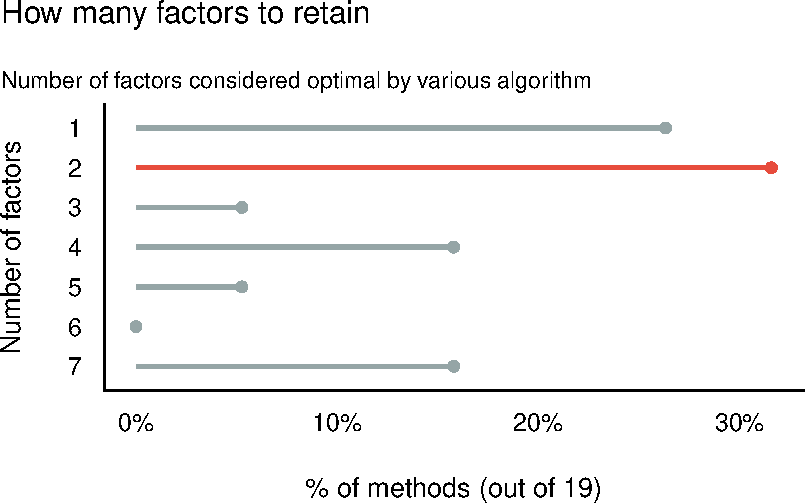
\includegraphics[keepaspectratio]{index_files/figure-pdf/unnamed-chunk-15-1.pdf}}

\begin{Shaded}
\begin{Highlighting}[]
\CommentTok{\# et visualiser le graphique des valeures propres}
\FunctionTok{SCREE\_PLOT}\NormalTok{(trainingpp, }\AttributeTok{corkind=}\StringTok{"spearman"}\NormalTok{, }\AttributeTok{verbose=}\NormalTok{T)}
\end{Highlighting}
\end{Shaded}

\pandocbounded{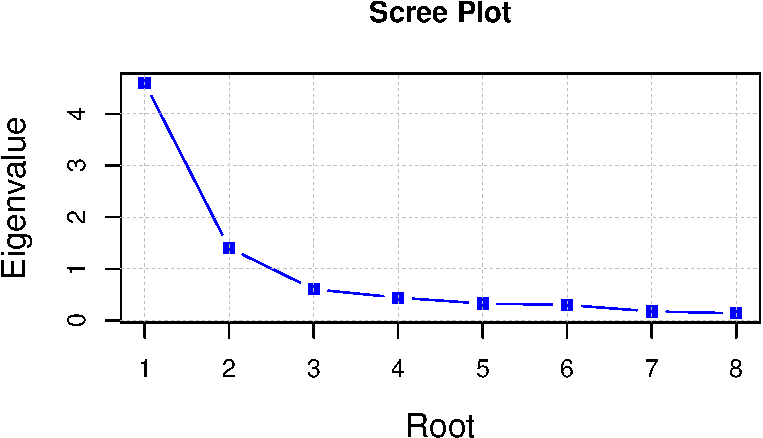
\includegraphics[keepaspectratio]{index_files/figure-pdf/unnamed-chunk-15-2.pdf}}

\begin{verbatim}


Scree Plot:

Specified kind of correlations for this analysis:  Spearman

Eigenvalues and Proportions of Total Variance Explained:

             Eig    prop     cum
Factor 1    4.60    0.58    0.58
Factor 2    1.40    0.18    0.75
Factor 3    0.61    0.08    0.83
Factor 4    0.44    0.06    0.88
Factor 5    0.33    0.04    0.92
Factor 6    0.30    0.04    0.96
Factor 7    0.18    0.02    0.98
Factor 8    0.14    0.02    1.00
\end{verbatim}

Ici nous observons très clairement grâce au graphique intitulé :
\emph{``How many factors to retain''} que la majorité des méthodes font
consensus sur trois facteurs latents (ligne rouge). Le tableau avec la
colonne \emph{n\_Methods} indique que 6 méthodes s'accordent sur une
structuration optimale des données en 2 facteurs latents. Toutefois,
dans ce même tableau, nous observons que 5 méthodes suggèrent une
structuration optimale des données en 1 facteur latent. En regard du
faible nombre de variables testées, ces solutions en 2 ou 1 facteurs
latents semblent pertinentes. C'est aussi une des forces de l'EFA de
pouvoir faire émerger un seul facteur latent global qui s'exprime au
travers de l'ensemble des variables observées testées. Ce peut être
intéressant de réaliser un comparatif afin de savoir comment se
structurent les données, si c'est plutôt en un ou en deux facteurs
latents.

\textbf{Ainsi quel est le meilleur modèle ?}

L'analyse factorielle confirmatoire (CFA) que nous allons présenter par
la suite permettra d'en décider. En attendant, nous pouvons lancer les
deux analyses !

Pour réaliser ces analyses il va falloir déterminer la méthode de
factorisation. C'est-à-dire définir sur quelle mesure nous nous basons
pour extraire les facteurs de notre ensemble de variables. Les méthodes
les plus couramment utilisées sont celles qui se basent soit sur le
maximum de vraisemblance (maximum likelihood), soit sur les méthodes des
moindres carrés (pondérés ou non) (weighted or unweighted least square)
(Tabachnick, B. G., \& Fidell, L. S., 2014). Dans notre exemple, après
observation des distributions des données, nous avons choisi de réaliser
les analyses avec la méthode de factorisation du maximum de
vraisemblance robuste (mlr). Cette méthode permet d'optimiser le calcul
des distances et la version robuste est adaptée à des données qui ne se
distribuent pas selon une loi normale (Kyriazos \& Poga, 2023). En
effet, les méthodes de maximum de vraisemblance reposent sur des
\emph{paramètres} tels que la moyenne. Si celle-ci est peu
représentative de la distribution des données étudiées, alors les
méthodes de maximum de vraisemblance sont à proscrire, car elles
produiront des résultats inadaptés et impertinents. C'est pour cela que
d'autres méthodes de factorisation existent, avec des méthodes de
calcul, soit qui ne sont pas basées sur des paramètres, soit pour
lesquelles une correction est appliquée afin de tenir compte de la
spécificité des données alors observées précédemment lors de
statistiques descriptives.

\begin{tcolorbox}[enhanced jigsaw, arc=.35mm, bottomrule=.15mm, bottomtitle=1mm, breakable, colback=white, colbacktitle=quarto-callout-note-color!10!white, colframe=quarto-callout-note-color-frame, coltitle=black, left=2mm, leftrule=.75mm, opacityback=0, opacitybacktitle=0.6, rightrule=.15mm, title=\textcolor{quarto-callout-note-color}{\faInfo}\hspace{0.5em}{Note}, titlerule=0mm, toprule=.15mm, toptitle=1mm]

\textbf{Aparte sur les rotations} :

Afin de pouvoir interpréter plus facilement les résultats des analyses
factorielles, il est nécessaire de faire appel à une méthode de rotation
(au-delà de 2 facteurs). Le principe de la rotation n'est pas de
modifier les relations obtenues entre les variables observées et les
facteurs, mais d'améliorer la lisibilité des résultats.

Il existe deux familles de rotation. Les rotations orthogonales et les
rotations obliques. Les rotations orthogonales doivent être privilégiées
lorsque l'on émet l'hypothèse que les facteurs obtenus ne sont pas
corrélés entre eux. Pour cette famille de rotation l'interprétation va
se centrer sur la relation de chaque variable observée avec chaque
facteur. Au contraire, les rotations obliques devront être employées
s'il est supposé que les facteurs obtenus sont corrélés entre eux. Dans
ce dernier cas, en plus de la matrice de corrélation calculée pour les
rotations orthogonales, une matrice supplémentaire incluant les
corrélations entre les facteurs va être produite. Il est à noter qu'en
SHS la plupart des factorisations impliquent une corrélation entre les
facteurs. Il est assez rare d'obtenir des facteurs qui ne soient pas du
tout corrélés dans ces disciplines. C'est pourquoi dans notre exemple
nous avons sélectionné une méthode de rotation oblique : \emph{promax}.

\end{tcolorbox}

\subsection{Réalisation des EFA}\label{ruxe9alisation-des-efa}

\textbf{1er modèle à un 1 facteur :}

\begin{Shaded}
\begin{Highlighting}[]
\CommentTok{\# Utilisation de mlr méthode considérée comme plus robuste même pour des données non{-}normales}

\CommentTok{\# Pour avoir mlr il faut utiliser la syntaxe ci{-}dessous :}
\CommentTok{\# Nous n\textquotesingle{}utilisons pas de méthode de rotation car nous testons la solution à 1 seul facteur}
\NormalTok{efa1immo }\OtherTok{\textless{}{-}}\NormalTok{ lavaan}\SpecialCharTok{::}\FunctionTok{efa}\NormalTok{(trainingpp, }\AttributeTok{nfactors =} \DecValTok{1}\NormalTok{, }\AttributeTok{estimator =} \StringTok{"MLR"}\NormalTok{)}

\FunctionTok{print}\NormalTok{(efa1immo)}
\end{Highlighting}
\end{Shaded}

\begin{verbatim}

                                     f1 
prix_med                          0.705*
perc_log_vac                     -0.532*
perc_maison                      -0.716*
perc_tiny_log                     0.761*
dens_pop                          0.755*
med_niveau_vis                    0.555*
part_agri_nb_emploi              -0.704*
part_cadre_profintellec_nbemploi  0.747*
\end{verbatim}

Avec un seul facteur toutes les variables observées corrèlent donc avec
un facteur latent. Dans notre cas on a toute une partie qui corrèle
positivement et l'autre négativement. Ainsi, le \emph{pourcentage de
petits logements}, la \emph{part des cadres dans l'emploi}, le
\emph{prix median du m²}, la \emph{densité de population} et le
\emph{niveau de vie médian} corrèlent positivement et à l'inverse, le
\emph{pourcentage de maison}, la \emph{part d'agriculteurs dans
l'emploi} et le \emph{pourcentage de logements vacants} corrèlent
négativement. Cela laisse à penser à une dichotomie qui pourrait être
ville / campagne. Ainsi le facteur latent exprimé par les huit variables
observées qui caractérisent les EPCI, serait une dimension sur le niveau
d'urbanité ou de ruralité. Toutefois nous ne pouvons l'affirmer à la
lecture de ces seuls résultats, des analyses complémentaires
permettraient d'éclairer ce point.

L'avantage de l'EFA c'est qu'une fois le facteur latent identifié, nous
pouvons, pour chaque individu obtenir un score sur ce facteur latent.
Dans notre exemple, vu la dimension spatiale des données il faudrait
ensuite les cartographier pour visualiser spatialement l'information.
L'intérêt des scores factoriels étant d'être ré-utilisés soit dans des
analyses complémentaires, soit directement pour comprendre la structure
des données. Dans notre cas, on pourrait s'en servir pour définir un
score d'urbanité et de ruralité puis le représenter.

\begin{Shaded}
\begin{Highlighting}[]
\CommentTok{\# Extraction des scores factoriels par observation}
\NormalTok{factor\_scores\_immo}\OtherTok{\textless{}{-}}\FunctionTok{predict}\NormalTok{(efa1immo)}

\CommentTok{\# Regardons  les 5 premières lignes}
\FunctionTok{head}\NormalTok{(factor\_scores\_immo, }\DecValTok{5}\NormalTok{)}
\end{Highlighting}
\end{Shaded}

\begin{verbatim}
               f1
[1,]  1.829256890
[2,]  0.003757627
[3,]  0.274161237
[4,] -0.342891760
[5,]  0.223668900
\end{verbatim}

\begin{Shaded}
\begin{Highlighting}[]
\CommentTok{\# Extraction des charges factorielles par variable}
\NormalTok{factor\_loadings\_immo }\OtherTok{\textless{}{-}}\NormalTok{ efa1immo}\SpecialCharTok{$}\NormalTok{loadings}

\CommentTok{\# Afficher les charges factorielles}
\FunctionTok{print}\NormalTok{(factor\_loadings\_immo)}
\end{Highlighting}
\end{Shaded}

\begin{verbatim}
                                     f1
prix_med                          0.705
perc_log_vac                     -0.532
perc_maison                      -0.716
perc_tiny_log                     0.761
dens_pop                          0.755
med_niveau_vis                    0.555
part_agri_nb_emploi              -0.704
part_cadre_profintellec_nbemploi  0.747
\end{verbatim}

\textbf{Testons le modèle à deux facteurs !}

\begin{Shaded}
\begin{Highlighting}[]
\CommentTok{\# Utilisation de mlr méthode considérée comme plus robuste même pour données non{-}normales}
\CommentTok{\# Utilisation d\textquotesingle{}une méthode de rotation promax car nous testons un modèle à2 facteurs}

\NormalTok{efa2immo }\OtherTok{\textless{}{-}}\NormalTok{ lavaan}\SpecialCharTok{::}\FunctionTok{efa}\NormalTok{(trainingpp, }\AttributeTok{nfactors =} \DecValTok{2}\NormalTok{, }\AttributeTok{estimator =} \StringTok{"MLR"}\NormalTok{, }\AttributeTok{rotation =} \StringTok{"promax"}\NormalTok{)}
\FunctionTok{print}\NormalTok{(efa2immo)}
\end{Highlighting}
\end{Shaded}

\begin{verbatim}

                                     f1     f2
prix_med                          0.944       
perc_log_vac                     -0.948      .
perc_maison                           . -0.631
perc_tiny_log                         .  1.096
dens_pop                                 0.688
med_niveau_vis                    0.665       
part_agri_nb_emploi                   . -0.491
part_cadre_profintellec_nbemploi         0.650
\end{verbatim}

Cette structure à deux facteurs permet de faire émerger en plus du
facteur latent, qui serait urbanité/ruralité (\emph{f2}), un autre
facteur représentant le côut de la vie (\emph{f1}). Au niveau de ce
facteur on observe une corrélation positive avec le prix \emph{médian de
l'immobilier au m²} et le \emph{niveau de vie médian}, et négative avec
le \emph{pourcentage de logements vacants}. Ainsi, les EPCI ayant un
score élevé sur ce facteur latent seraient les EPCI où le niveau de vie
médian et le prix de l'immobilier seraient le plus élévé.

Extraction des charges factorielles par variable :

\begin{Shaded}
\begin{Highlighting}[]
\NormalTok{factor\_loadings\_immo2 }\OtherTok{\textless{}{-}}\NormalTok{ efa2immo}\SpecialCharTok{$}\NormalTok{loadings}

\CommentTok{\# Afficher les charges factorielles}
\FunctionTok{print}\NormalTok{(factor\_loadings\_immo2)}
\end{Highlighting}
\end{Shaded}

\begin{verbatim}
                                     f1     f2
prix_med                          0.944 -0.013
perc_log_vac                     -0.948  0.252
perc_maison                      -0.167 -0.631
perc_tiny_log                    -0.263  1.096
dens_pop                          0.086  0.688
med_niveau_vis                    0.665  0.001
part_agri_nb_emploi              -0.209 -0.491
part_cadre_profintellec_nbemploi  0.096  0.650
\end{verbatim}

Une fois de plus nous pouvons extraire les scores de ces deux facteurs
latents de ce second modèle.

\begin{Shaded}
\begin{Highlighting}[]
\CommentTok{\# Extraction des scores factoriels par observation}
\NormalTok{factor\_scores\_immo2}\OtherTok{\textless{}{-}}\FunctionTok{predict}\NormalTok{(efa2immo)}

\CommentTok{\# Regardons  les 5 premières lignes}
\FunctionTok{head}\NormalTok{(factor\_scores\_immo2, }\DecValTok{5}\NormalTok{)}
\end{Highlighting}
\end{Shaded}

\begin{verbatim}
             f1         f2
[1,]  1.3347563  2.3713092
[2,]  0.2115704 -0.1939248
[3,] -0.7920895  0.6989897
[4,] -0.2897778 -0.4770623
[5,]  0.6513887 -0.2907544
\end{verbatim}

Il est tout à fait possible dans le cadre de l'EFA d'emprunter une
représentation classique de l'ACP (le scatter plot) pour représenter les
variables et leurs charges factorielles. Cette représentation peut
s'avérer également utile pour mieux comprendre les facteurs latents.
Voici un exemple de représentation avec la structuration en 2 facteurs
latents.

\begin{Shaded}
\begin{Highlighting}[]
\CommentTok{\# Graphique}


\CommentTok{\# Extraire les charges factorielles}
\NormalTok{factor\_loadings\_immo2 }\OtherTok{\textless{}{-}}\NormalTok{ efa2immo}\SpecialCharTok{$}\NormalTok{loadings}

\CommentTok{\# transformer les charges factorielles dans un data frame}
\NormalTok{factor\_loadings\_dfimmo2 }\OtherTok{\textless{}{-}} \FunctionTok{as.data.frame}\NormalTok{(factor\_loadings\_immo2)}

\CommentTok{\# Renommer les colonnes}
\FunctionTok{colnames}\NormalTok{(factor\_loadings\_dfimmo2) }\OtherTok{\textless{}{-}} \FunctionTok{c}\NormalTok{(}\StringTok{"Factor"}\NormalTok{, }\StringTok{"Loading"}\NormalTok{)}

\CommentTok{\#  Ajouter une variables pour identifier nos charges factorielles}
\NormalTok{factor\_loadings\_dfimmo2}\SpecialCharTok{$}\NormalTok{Item }\OtherTok{\textless{}{-}} \FunctionTok{rownames}\NormalTok{(factor\_loadings\_dfimmo2)}

\CommentTok{\# charger ggplot2}
\FunctionTok{library}\NormalTok{(ggplot2)}

\CommentTok{\# Réaliser un graphique des charges factorielles}
\FunctionTok{ggplot}\NormalTok{(factor\_loadings\_dfimmo2, }\FunctionTok{aes}\NormalTok{(}\AttributeTok{x =}\NormalTok{ Factor, }\AttributeTok{y =}\NormalTok{ Loading, }\AttributeTok{label =}\NormalTok{ Item)) }\SpecialCharTok{+}
  \FunctionTok{geom\_point}\NormalTok{() }\SpecialCharTok{+}
  \FunctionTok{geom\_text}\NormalTok{(}\AttributeTok{size =} \DecValTok{3}\NormalTok{, }\AttributeTok{hjust =} \SpecialCharTok{{-}}\FloatTok{0.1}\NormalTok{) }\SpecialCharTok{+}
  \FunctionTok{labs}\NormalTok{(}\AttributeTok{x =} \StringTok{"Factor"}\NormalTok{, }\AttributeTok{y =} \StringTok{"Loading"}\NormalTok{, }\AttributeTok{title =} \StringTok{"Factor Loadings Plot"}\NormalTok{) }\SpecialCharTok{+}
  \FunctionTok{theme\_minimal}\NormalTok{()}
\end{Highlighting}
\end{Shaded}

\pandocbounded{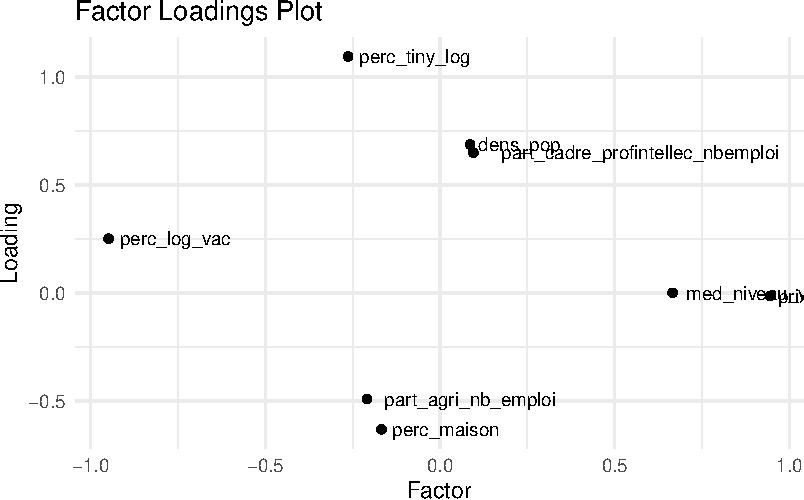
\includegraphics[keepaspectratio]{index_files/figure-pdf/unnamed-chunk-21-1.pdf}}

Cette représentation graphique permet bien d'observer la proximité entre
les variables observées précédemment, comme par exemple entre la
\emph{part d'agriculteurs} et le \emph{pourcentage de maison} ou encore
entre la \emph{densité de population} et la \emph{part de cadre}.

\subsection{Conclusion sur les EFA}\label{conclusion-sur-les-efa}

Ces EFA réalisées sur la moitié de l'échantillon de données indiquent la
possibilité d'envisager un modèle en un facteur latent (rural/urbain) ou
un modèle en deux facteurs latents (rural/urbain ; coût de la vie).

Les structures obtenues, suite aux analyses factorielles exploratoires
menées, s'ajustent-elles aux données d'un autre échantillon (tel que la
base \emph{testp}) ? Quel est le meilleur modèle celui à 1 ou 2 facteurs
? Afin de répondre à cette question et d'éprouver le modèle théorique
envisagé, il est nécessaire de réaliser des analyses factorielles
confirmatoires.

\section{L'Analyse factorielle
confirmatoire}\label{lanalyse-factorielle-confirmatoire}

L'analyse factorielle confirmatoire est une technique statistique
utilisée pour tester un modèle factoriel.

Si dans le cas de l'EFA les facteurs latents sont identifiés dans une
démarche exploratoire à partir des données, dans le cadre de l'analyse
factorielle confirmatoire il s'agira au contraire de tester un modèle
avec des hypothèses pré-établies sur la structuration des données par
des facteurs latents pré-supposés. L'idée dans une analyse factorielle
confirmatoire est d'imposer une structure aux données et d'étudier dans
quelle mesure les données vont correspondre à cette structure
prédéfinie. L'objectif de la CFA est de mesurer l'ajustement d'un modèle
aux données présentées. C'est en ce sens que cette analyse est
confirmatoire.

\subsection{Les étapes de la CFA}\label{les-uxe9tapes-de-la-cfa}

Nous étudions comment un modèle pré-établi dans le cadre d'une théorie,
ou suite à une première analyse statistique sur des données, est
confirmée par les données observées. La réalisation d'une CFA nécessite
le suivi des étapes successives, suivantes :

\begin{itemize}
\item
  1- \textbf{Définir un modèle Préalable} : Spécifier un modèle
  factoriel a priori, indiquant la relation entre les variables
  observées et les facteurs latents que nous supposons. Le modèle peut
  également inclure des relations entre les facteurs latents.
\item
  2- \textbf{Lire les critères d'ajustement} : La qualité et
  l'ajustement du modèle sont évalués en utilisant divers critères
  statistiques évaluant la position du modèle entre un modèle nul (sans
  aucun lien - le modèle ne s'ajuste pas aux données) et un modèle
  saturé (avec des liens très maximum partout - le modèle correspond
  parfaitement aux données). Les indices les plus couramment utilisés
  sont notamment : le chi², le RMSEA, le CFI, etc.
\item
  3- \textbf{Obtenir les estimations des paramètres} : Après avoir
  évalué une bonne qualité d'ajustement du modèle testé aux données
  présentées, il est nécessaire de vérifier l'importance et le sens des
  relations entre les variables observées et la ou les facteur(s)
  latent(s). Les différents paramètres de l'analyse factorielle
  confirmatoire (charges factorielles, covariances entre les facteurs
  latents\ldots) sont estimés à l'aide des données observées. L'objectif
  de l'analyse étant d'obtenir des estimations qui maximisent
  l'ajustement entre les données observées et le modèle.
\item
  4- \textbf{Interpréter les résultats} : Les charges factorielles
  indiquent la force et la direction de la relation entre chaque
  variable observée et son facteur latent correspondant. A partir de ces
  indications, nous pouvons interpréter les résultats et vérifier si la
  structure obtenue est bien dans le même sens que celle envisagée.
\item
  5- \textbf{Modifier le modèle} : Si le modèle ne s'ajuste pas bien
  (que les indices d'ajustement ne sont pas satisfaisants), des
  modifications peuvent être apportées, comme la suppression ou l'ajout
  de liens entre les facteurs et les variables observées, pour améliorer
  l'ajustement. Attention toutefois à rester dans un cadre théorique
  cohérent et ne pas tester des liens qui n'ont pas de sens.
\end{itemize}

Tout l'enjeu en cas de non ajustement du modèle va être de comprendre et
d'analyser pourquoi le modèle ne s'ajuste pas. Cela peut venir d'un
modèle théorique qui n'est pas adapté aux données observées ou à des
variations entre la première analyse, qui permet d'établir un premier
modèle, et sa confirmation via l'analyse factorielle confirmatoire.

\subsection{L'analyse factorielle confirmatoire en pratique : Exemple
sur le prix de l'immobilier - Quel modèle choisir
?}\label{lanalyse-factorielle-confirmatoire-en-pratique-exemple-sur-le-prix-de-limmobilier---quel-moduxe8le-choisir}

L'analyse factorielle confirmatoire fait partie du champ des équations
structurelles, sa mise en oeuvre se fait très bien sur R. L'avantage des
équations structurelles c'est qu'à la manière de l'ACP nous pourrons
représenter graphiquement les modèles obtenus.

\subsubsection{Définir un modèle
Préalable}\label{duxe9finir-un-moduxe8le-pruxe9alable}

Cette étape a été réalisée précédemment lors de l'EFA et deux structures
possibles ont été mises en évidence. La première structure comporte un
seul facteur latent répartissant les éléments relatifs au prix de
l'immobilier selon un critère opposant ruralité/urbanité. Le second
modèle structurant les données en deux facteurs latents dont l'un
toujours sur l'opposition ruralité/urbanité et l'autre portant sur le
coût de la vie.

Nous allons à présent réaliser deux analyses factorielles confirmatoires
afin de sélectionner le modèle qui structure le mieux les données entre
celui en 1 facteur latent et celui en 2 facteurs latents.

\subsubsection{Réalisation des CFA}\label{ruxe9alisation-des-cfa}

Les CFA sont réalisées sur la base de données \emph{testpp}, afin de
tester la structure factorielle sur un autre échantillon que celui qui a
été utilisé lors des EFA, comme préconisé dans la littérature
scientifique.

\begin{Shaded}
\begin{Highlighting}[]
\FunctionTok{library}\NormalTok{(lavaan)}

\FunctionTok{attach}\NormalTok{(testpp) }\CommentTok{\# nécessaire à cause du package lavaan}

\CommentTok{\# modèle à 1 facteur}
\NormalTok{model1F}\OtherTok{\textless{}{-}} \StringTok{\textquotesingle{}F1 =\textasciitilde{} prix\_med + perc\_log\_vac + perc\_maison + perc\_tiny\_log + dens\_pop + med\_niveau\_vis + part\_agri\_nb\_emploi + part\_cadre\_profintellec\_nbemploi\textquotesingle{}}

\NormalTok{fact\_1immo }\OtherTok{\textless{}{-}} \FunctionTok{cfa}\NormalTok{(model1F, }\AttributeTok{std.lv=}\NormalTok{T, }\AttributeTok{estimator=}\StringTok{"MLR"}\NormalTok{, }\AttributeTok{data=}\NormalTok{testpp)}

\CommentTok{\# modèle à 2 facteurs}
\NormalTok{model2F}\OtherTok{\textless{}{-}} \StringTok{\textquotesingle{}F1 =\textasciitilde{} prix\_med + perc\_log\_vac + med\_niveau\_vis}
\StringTok{           F2 =\textasciitilde{} perc\_maison + perc\_tiny\_log + dens\_pop + part\_agri\_nb\_emploi + part\_cadre\_profintellec\_nbemploi\textquotesingle{}}

\NormalTok{fact\_2immo }\OtherTok{\textless{}{-}} \FunctionTok{cfa}\NormalTok{(model2F, }\AttributeTok{std.lv=}\NormalTok{T, }\AttributeTok{estimator=}\StringTok{"MLR"}\NormalTok{, }\AttributeTok{data=}\NormalTok{testpp)}
\end{Highlighting}
\end{Shaded}

\subsubsection{Lire les critères d'ajustement (du modèle aux
données)}\label{lire-les-crituxe8res-dajustement-du-moduxe8le-aux-donnuxe9es}

Attention les sorties d'un modèle d'analyse factorielle confirmatoire
sont nombreuses, nous les détaillons ici pour en avoir une première
lecture mais leurs analyses se feront véritablement à l'aide d'autres
fonctions. Il faut retenir que deux grandes étapes seront à évaluer dans
cet ordre :

\begin{itemize}
\tightlist
\item
  l'adéquation du modèle proposé aux données (avec la vérification des
  indices d'ajustement au modèle) - \emph{on parle de modèle de mesure}
\item
  et si le modèle s'ajuste correctement nous pourrons alors étudier la
  structure de celui-ci par la force et le signe des saturations
  obtenues à l'aide de l'estimation des paramètres - \emph{on parle
  alors de modèle de structure}.
\end{itemize}

Vérifions à présent la première étape, qui correspond à cette partie, à
savoir l'ajustement du modèle aux données. Tout notre enjeu ici va être
de comparer les deux modèles et de choisir celui qui s'ajuste le mieux
aux données. Pour ce faire nous pouvons comparer les deux modèles sur
différents indices d'ajustement. La fonction \texttt{interpret()} permet
d'évaluer dix indices d'ajustement les plus couramment employés dans la
littérature scientifique.

\begin{Shaded}
\begin{Highlighting}[]
\CommentTok{\# Pour comparer les modèles à l\textquotesingle{}aide des indices tel que l\textquotesingle{}AIC, le RMSEA, R2...}
\NormalTok{performance}\SpecialCharTok{::}\FunctionTok{compare\_performance}\NormalTok{(fact\_1immo, fact\_2immo, }\AttributeTok{verbose =} \ConstantTok{FALSE}\NormalTok{)}
\end{Highlighting}
\end{Shaded}

\begin{verbatim}
# Comparison of Model Performance Indices

Name       |  Model |    Chi2 | Chi2_df | p (Chi2) | Baseline(28)
-----------------------------------------------------------------
fact_1immo | lavaan | 852.714 |      20 |   < .001 |     2751.450
fact_2immo | lavaan | 319.597 |      19 |   < .001 |     2751.450

Name       | p (Baseline) |   GFI |  AGFI |   NFI |  NNFI |   CFI | RMSEA
-------------------------------------------------------------------------
fact_1immo |       < .001 | 0.735 | 0.515 | 0.690 | 0.572 | 0.694 | 0.265
fact_2immo |       < .001 | 0.892 | 0.783 | 0.884 | 0.837 | 0.890 | 0.163

Name       |      RMSEA  CI | p (RMSEA) |   RMR |  SRMR |   RFI |  PNFI |   IFI
-------------------------------------------------------------------------------
fact_1immo | [0.250, 0.280] |    < .001 | 0.104 | 0.123 | 0.566 | 0.493 | 0.695
fact_2immo | [0.148, 0.179] |    < .001 | 0.057 | 0.066 | 0.829 | 0.600 | 0.890

Name       |   RNI | Loglikelihood |  AIC (weights) |  BIC (weights) | BIC_adjusted
-----------------------------------------------------------------------------------
fact_1immo | 0.694 |     -4904.989 | 9842.0 (<.001) | 9912.1 (<.001) |     9861.346
fact_2immo | 0.890 |     -4638.430 | 9310.9 (>.999) | 9385.4 (>.999) |     9331.439
\end{verbatim}

\begin{Shaded}
\begin{Highlighting}[]
\CommentTok{\# Une autre manière de visualiser très utile.}
\NormalTok{effectsize}\SpecialCharTok{::}\FunctionTok{interpret}\NormalTok{(fact\_1immo)}
\end{Highlighting}
\end{Shaded}

\begin{verbatim}
    Name     Value Threshold Interpretation
1    GFI 0.7350803      0.95           poor
2   AGFI 0.5149939      0.90           poor
3    NFI 0.6900854      0.90           poor
4   NNFI 0.5719399      0.90           poor
5    CFI 0.6942428      0.90           poor
6  RMSEA 0.2649755      0.05           poor
7   SRMR 0.1229386      0.08           poor
8    RFI 0.5661196      0.90           poor
9   PNFI 0.4929182      0.50           poor
10   IFI 0.6951383      0.90           poor
\end{verbatim}

\begin{Shaded}
\begin{Highlighting}[]
\NormalTok{effectsize}\SpecialCharTok{::}\FunctionTok{interpret}\NormalTok{(fact\_2immo)}
\end{Highlighting}
\end{Shaded}

\begin{verbatim}
    Name      Value Threshold Interpretation
1    GFI 0.89178269      0.95           poor
2   AGFI 0.78297251      0.90           poor
3    NFI 0.88384431      0.90           poor
4   NNFI 0.83734440      0.90           poor
5    CFI 0.88962655      0.90           poor
6  RMSEA 0.16333823      0.05           poor
7   SRMR 0.06563246      0.08   satisfactory
8    RFI 0.82882320      0.90           poor
9   PNFI 0.59975150      0.50   satisfactory
10   IFI 0.88999010      0.90           poor
\end{verbatim}

Dans les deux configurations testées, l'analyse factorielle
confirmatoire présente un ajustement des modèles aux données
\emph{``testpp''} plutôt mauvais. Pour le deuxième modèle toutefois, 2
indices sont considérés comme satisfaisants et 3 indices ont des valeurs
très proches des seuils (NFI : 0.8838; CFI : 0.8896 ; IFI : 0.8899). Ces
indices indiquent l'écart entre un modèle nul (rien n'est lié) et un
modèle saturé (tout est lié avec des coefficients à 1). Le fait que ces
indices aient des valeurs de 0.88 ou 0.89 et non de 0.90 n'est pas
particulièrement problématique.

Concrètement, le deuxième modèle testé, avec 2 facteurs latents
permettrait de mieux rendre compte de la complexité des données.
Celui-ci s'ajustant le mieux aux données.

\begin{tcolorbox}[enhanced jigsaw, arc=.35mm, bottomrule=.15mm, bottomtitle=1mm, breakable, colback=white, colbacktitle=quarto-callout-note-color!10!white, colframe=quarto-callout-note-color-frame, coltitle=black, left=2mm, leftrule=.75mm, opacityback=0, opacitybacktitle=0.6, rightrule=.15mm, title=\textcolor{quarto-callout-note-color}{\faInfo}\hspace{0.5em}{Note}, titlerule=0mm, toprule=.15mm, toptitle=1mm]

La fonction \texttt{interpret()} donne des résultats pour 10 indices
d'ajustement du modèle testé aux données de l'échantillon présenté.
Toutefois, ces différents indices ont été proposés au fur et à mesure du
développement des modèles en équations structurelles et, s'ils ne
testent pas exactement la même chose, ils permettent de rendre compte de
l'ajustement d'un modèle aux données présentées. Il n'est pas nécessaire
que l'ensemble des indices présentés soient satisfaisant pour envisager
un bon ajustement. Dans la littérature, certains indices sont
sélectionnés et tous ne sont pas présentés. De plus, une utilisation
trop contrainte des seuils augmente la probabilité de faux négatifs,
c'est-à-dire de considérer qu'un modèle ne s'ajusterait pas aux données
alors que si (Hooper et al., 2008). Prenons l'exemple d'un indice très
cité et présenté dans la littérature tel que le CFI \textbf{Comparative
Fit Indice}. Que fait-il exactement ? Il compare le modèle d'intérêt
avec un modèle restreint qui sert de base. Itération de modèles entre le
pire (modèle nul -- à 0) et le parfait (voir modèle saturé - 1) et le
CFI indique où se situe le modèle d'intérêt (le notre) sur ce continuum.
Le seuil communément accepté de .95 indique une réduction de l'erreur,
par rapport au modèle nul, de 95\%. Le modèle nul étant un modèle où
toutes les relations entre les variables sont rapportées à 0. Donc en
gros notre modèle s'ajuste à nos données avec un risque de 5\% que ce
soit du au hasard. Quel que soit le contexte on est satisfait d'avoir
une réduction de l'erreur de 95\%. Donc plus le seuil est inférieur à
.95, plus le risque que l'ajustement soit du au hasard augmente. (Van
Laar, S., \& Braeken, J., 2021).

\end{tcolorbox}

\subsubsection{Obtenir les estimations des
paramètres}\label{obtenir-les-estimations-des-paramuxe8tres}

Après avoir vérifié l'ajustement du modèle aux données, il est à présent
nécessaire de comprendre si le modèle envisagé a bien des relations de
l'intensité et du sens prévues initialement. Ceci est possible grâce à
la lecture des paramètres telles que les charges factorielles.

La qualité des ajustements, évaluée précédemment, invite à ne
s'intéresser qu'au modèle à deux facteurs latents, toutefois, dans un
but pédagogique nous présenterons la composition des structures des deux
modèles testés.

La composition des modèles testés s'obtient en faisant appel à la
fonction \texttt{summary()} qu'on applique aux objets contenant les
données des CFA alors réalisées précédemment, à savoir
\emph{fact\_1immo} et \emph{fact\_2immo}.

\begin{Shaded}
\begin{Highlighting}[]
\NormalTok{res\_fact1immo }\OtherTok{\textless{}{-}} \FunctionTok{summary}\NormalTok{(fact\_1immo, }\AttributeTok{standardized=}\NormalTok{T, }\AttributeTok{modindices =}\NormalTok{ T, }\AttributeTok{fit.measures=}\NormalTok{T, }\AttributeTok{rsquare=}\NormalTok{T)}

\NormalTok{res\_fact2immo }\OtherTok{\textless{}{-}} \FunctionTok{summary}\NormalTok{(fact\_2immo, }\AttributeTok{standardized=}\NormalTok{T, }\AttributeTok{modindices =}\NormalTok{ T, }\AttributeTok{fit.measures=}\NormalTok{T, }\AttributeTok{rsquare=}\NormalTok{T)}
\end{Highlighting}
\end{Shaded}

Voici, pour exemple, la sortie brute de \texttt{summary()} du modèle en
2 facteurs. On y retrouve également les R2.

\begin{Shaded}
\begin{Highlighting}[]
\CommentTok{\# Exemple pour le modèle à 2 facteurs}

\CommentTok{\# Récupérer les résultats de l\textquotesingle{}output}
\NormalTok{cfa\_output }\OtherTok{\textless{}{-}} \FunctionTok{capture.output}\NormalTok{(res\_fact2immo)}

\CommentTok{\# Placer les résultats dans une sortie déroulante pour améliorer la lisibilité}
\FunctionTok{cat}\NormalTok{(}
  \StringTok{\textquotesingle{}\textless{}div style="max{-}height: 400px; overflow{-}y: auto; border: 1px solid \#ccc; padding: 10px;"\textgreater{}\textquotesingle{}}\NormalTok{,}
  \StringTok{\textquotesingle{}\textless{}pre style="margin: 0; font{-}family: monospace; font{-}size: 14px;"\textgreater{}\textquotesingle{}}\NormalTok{,}
  \FunctionTok{paste}\NormalTok{(cfa\_output, }\AttributeTok{collapse =} \StringTok{"}\SpecialCharTok{\textbackslash{}n}\StringTok{"}\NormalTok{),}
  \StringTok{\textquotesingle{}\textless{}/pre\textgreater{}\textquotesingle{}}\NormalTok{,}
  \StringTok{\textquotesingle{}\textless{}/div\textgreater{}\textquotesingle{}}
\NormalTok{)}
\end{Highlighting}
\end{Shaded}

\begin{itemize}
\tightlist
\item
  header : contient des éléments contextuels sur la fonction (version du
  package\ldots) ainsi que les mesures d'ajustement si
  \texttt{fitMeasures=TRUE}
\item
  optim : liste d'information concernant l'optimisation du modèle
\item
  data : contient des éléments sur les données
\item
  test : les résultats des différents tests
\item
  fit : les résultats des différents test d'ajustement du modèle
\item
  pe : les différents paramètres des relations au sein du modèle sous la
  forme d'un data frame des facteurs latent et de la variance
\item
  \emph{mi : si modindices=TRUE}, il s'agit des suggestions proposées
  par la fonction pour améliorer le modèle si l'ajustement n'est pas
  optimal.
\end{itemize}

\subsection{Précaution d'utilisation}\label{pruxe9caution-dutilisation}

ATTENTION cette option \emph{modindices=TRUE} est à utiliser avec
précautions. L'idée ici est bien de tester un modèle théorique
pré-établi et donc chaque modification proposée qui seraient ajoutées au
modèle final doit pouvoir se justifier théoriquement. La corrélation de
l'ensemble des erreurs de mesure ensemble, comme c'est souvent proposé
par cette option, est difficile à justifier dans un modèle théorique
pré-établi.

Nous observons, dans la sortie brute pour le modèle à 2 facteurs, dans
la partie du tableau intitulée \emph{Latent Variables} et dans la
colonne \emph{Estimate} que les saturations les plus élevées sont pour
le facteur 1 (F1) \emph{le prix médian de l'immobilier au m²}, alors que
pour le facteur 2 (F2) il s'agit du \emph{pourcentage de petits
logements} (qui corrèle négativement sur ce facteur 2) et \emph{le
pourcentage de maison} (qui lui corrèle positivement sur ce facteur 2).
Une seule saturation est faible (inférieure à 0.30), les autres
apportent une part de variance significative au modèle.

\subsubsection{Interpréter les
résultats}\label{interpruxe9ter-les-ruxe9sultats}

Afin d'aider lecture des résultats obtenus, nous pouvons représenter
graphiquement chacun des modèles théoriques testés et leurs
structurations sur l'ensemble de données testé. Ceci permet de voir
rapidement l'intensité et le sens des relations entre les différentes
variables observées et le ou les facteur(s) latent(s).

Voici donc les représentations graphiques des CFA, qui obéissent à un
certain nombre de codes visuels qu'il est important de respecter. Ces
codes visuels sont mobilisés dans toutes les représentations de modèles
en équations structurelles :

\begin{itemize}
\tightlist
\item
  Les rectangles renvoient aux variables observées
\item
  Les ellipses aux variables latentes,
\item
  Les doubles flèches associées aux rectangles et aux ellipses à
  l'erreur de chaque variable.
\end{itemize}

Les couleurs vertes et rouges renvoient au signe de la corrélation et
l'épaisseur à la force de la corrélation entre les variables et les
facteurs.

Petite précision sur l'erreur : Il s'agit de la part de variance qui
n'est pas expliquée par le modèle.

Représentations graphiques des CFA

\pandocbounded{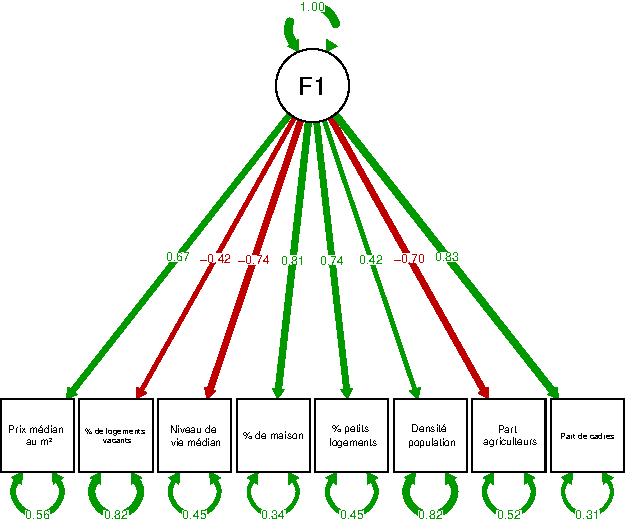
\includegraphics[keepaspectratio]{index_files/figure-pdf/unnamed-chunk-27-1.pdf}}

Uniquement le code pour le modèle à 2 facteurs est représenté afin de ne
pas alourdir la lecture.

\begin{Shaded}
\begin{Highlighting}[]
\NormalTok{new\_labels2 }\OtherTok{\textless{}{-}} \FunctionTok{list}\NormalTok{(}
  \StringTok{"prix\_med"} \OtherTok{=} \StringTok{"Prix médian }\SpecialCharTok{\textbackslash{}n}\StringTok{ au m²"}\NormalTok{,}
  \StringTok{"perc\_log\_vac"} \OtherTok{=} \StringTok{"\% de logements }\SpecialCharTok{\textbackslash{}n}\StringTok{ vacants"}\NormalTok{,}
  \StringTok{"med\_niveau\_vis"} \OtherTok{=} \StringTok{"Niveau de }\SpecialCharTok{\textbackslash{}n}\StringTok{ vie médian"}\NormalTok{,}
  \StringTok{"perc\_maison"} \OtherTok{=} \StringTok{"\% de maison"}\NormalTok{,}
  \StringTok{"perc\_tiny\_log"} \OtherTok{=} \StringTok{"\% petits }\SpecialCharTok{\textbackslash{}n}\StringTok{ logements"}\NormalTok{,}
  \StringTok{"dens\_pop"} \OtherTok{=} \StringTok{"Densité }\SpecialCharTok{\textbackslash{}n}\StringTok{ population"}\NormalTok{,}
  \StringTok{"part\_agri\_nb\_emploi"} \OtherTok{=} \StringTok{"Part }\SpecialCharTok{\textbackslash{}n}\StringTok{ agriculteurs"}\NormalTok{,}
  \StringTok{"part\_cadre\_profintellec\_nbemploi"} \OtherTok{=} \StringTok{"Part de cadres"}\NormalTok{,}
  \StringTok{"F1"} \OtherTok{=} \StringTok{"F1"}\NormalTok{,}
  \StringTok{"F2"} \OtherTok{=} \StringTok{"F2"}\NormalTok{)}

\NormalTok{semPlot}\SpecialCharTok{::}\FunctionTok{semPaths}\NormalTok{(fact\_2immo, }\StringTok{"std"}\NormalTok{,}
             \AttributeTok{sizeMan =} \DecValTok{10}\NormalTok{, }\AttributeTok{sizeInt =} \DecValTok{10}\NormalTok{, }\AttributeTok{sizeLat =} \DecValTok{10}\NormalTok{,}
             \AttributeTok{edge.label.cex=}\FloatTok{0.8}\NormalTok{, }\AttributeTok{label.cexs =} \DecValTok{2}\NormalTok{, }\AttributeTok{label.rotate =} \DecValTok{0}\NormalTok{, }\AttributeTok{label.font =} \FloatTok{6.5}\NormalTok{, }\AttributeTok{label.color =} \StringTok{"black"}\NormalTok{,}
             \AttributeTok{nodeLabels =}\NormalTok{ new\_labels2,}
             \AttributeTok{fade=}\ConstantTok{FALSE}\NormalTok{)}
\end{Highlighting}
\end{Shaded}

\pandocbounded{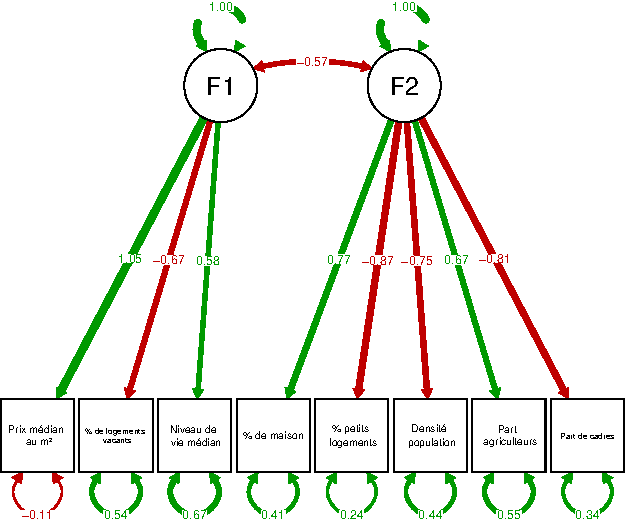
\includegraphics[keepaspectratio]{index_files/figure-pdf/unnamed-chunk-28-1.pdf}}

Les représentations graphiques des modèles à 1 facteur et à 2 facteurs
permettent d'illustrer ce que nous observions précédemment à la lecture
des paramètres et des charges factorielles. C'est-à-dire que les plus
élevées sont bien toujours celles associées au \emph{pourcentage de
petits logements} pour le facteur 2 (F2) et au \emph{prix médian de
l'immobilier au m²} pour le facteur 1 (F1). L'analyse factorielle
confirmatoire vient confirmer que le modèle en deux facteurs latents
structure les données de façon pertinente. La lecture des graphiques
avec la force des liens et leurs sens confirme qu'il s'agit bien de la
même structure, les mêmes variables sont influencées aussi fortement et
dans le même sens par les facteurs latents qu'observé lors de l'EFA.

\subsubsection{Modifier le modèle}\label{modifier-le-moduxe8le}

Nous l'avons déjà observé précédemment, la fonction \texttt{summary()}
appliquée à l'objet contenant le modèle de CFA comprend une instruction
proposant de modifier le modèle afin de l'améliorer, il s'agit de
l'instruction \emph{modindices=TRUE}. Cette option peut s'avérer utile
mais à utiliser avec précaution pour ne pas s'éloigner du modèle
théorique alors envisagé en premier lieu et que le modèle testé conserve
tout son sens théorique.

Le package Lavaan, fait également quelques propositions pour améliorer
le modèle. Théoriquement, en tenant compte de toutes ces propositions,
le modèle s'ajusterait parfaitement, mais on serait dans un cas évident
de sur-ajustement aux données. En revanche, cela peut être intéressant
d'en prendre connaissance afin de vérifier qu'aucune relation n'ait été
oubliée et qui permettrait d'améliorer significativement le modèle.
Cette relation doit bien évidemment faire sens théoriquement. La syntaxe
utilisée est celle du package lavaan, on peut en trouver une traduction
\href{https://lavaan.ugent.be/tutorial/syntax1.html}{ici}

Pour améliorer la lisibilité de l'article, l'instruction de modification
des indices ne sera présentée que sur le modèle à 2 facteurs.

\begin{Shaded}
\begin{Highlighting}[]
\FunctionTok{modindices}\NormalTok{(fact\_2immo) }\SpecialCharTok{\%\textgreater{}\%} \FunctionTok{arrange}\NormalTok{(}\SpecialCharTok{{-}}\NormalTok{mi) }\SpecialCharTok{\%\textgreater{}\%} \FunctionTok{head}\NormalTok{(}\DecValTok{20}\NormalTok{)}
\end{Highlighting}
\end{Shaded}

\begin{verbatim}
                   lhs op                              rhs     mi    epc
1                   F1 =~                    perc_tiny_log 63.560 -0.220
2          perc_maison ~~ part_cadre_profintellec_nbemploi 57.672  0.135
3       med_niveau_vis ~~ part_cadre_profintellec_nbemploi 54.545  0.138
4          perc_maison ~~                    perc_tiny_log 39.987 -0.113
5       med_niveau_vis ~~                      perc_maison 36.013  0.126
6         perc_log_vac ~~                    perc_tiny_log 34.577  0.090
7             prix_med ~~                      perc_maison 34.347 -0.073
8        perc_tiny_log ~~              part_agri_nb_emploi 29.203  0.106
9                   F1 =~                      perc_maison 19.947 -0.141
10 part_agri_nb_emploi ~~ part_cadre_profintellec_nbemploi 19.742 -0.089
11        perc_log_vac ~~              part_agri_nb_emploi 14.195  0.083
12                  F2 =~                         prix_med 12.391 -0.209
13        perc_log_vac ~~                   med_niveau_vis 12.391 -0.107
14         perc_maison ~~                         dens_pop 11.718  0.026
15      med_niveau_vis ~~                    perc_tiny_log 11.410 -0.059
16                  F2 =~                     perc_log_vac 10.684 -0.152
17            prix_med ~~                   med_niveau_vis 10.683 -0.138
18       perc_tiny_log ~~                         dens_pop 10.243  0.022
19                  F1 =~ part_cadre_profintellec_nbemploi  9.279  0.088
20      med_niveau_vis ~~              part_agri_nb_emploi  8.459 -0.073
   sepc.lv sepc.all sepc.nox
1   -0.220   -0.243   -0.243
2    0.135    0.429    0.429
3    0.138    0.329    0.329
4   -0.113   -0.418   -0.418
5    0.126    0.259    0.259
6    0.090    0.279    0.279
7   -0.073   -0.439   -0.439
8    0.106    0.314    0.314
9   -0.141   -0.150   -0.150
10  -0.089   -0.228   -0.228
11   0.083    0.153    0.153
12  -0.209   -0.252   -0.252
13  -0.107   -0.185   -0.185
14   0.026    0.176    0.176
15  -0.059   -0.163   -0.163
16  -0.152   -0.156   -0.156
17  -0.138   -0.625   -0.625
18   0.022    0.205    0.205
19   0.088    0.098    0.098
20  -0.073   -0.121   -0.121
\end{verbatim}

\section*{Conclusion}\label{conclusion}
\addcontentsline{toc}{section}{Conclusion}

Nous avons ainsi présenté pas à pas un exemple d'utilisation de l'EFA et
en suivant de la CFA. L'idée était de présenter une méthode ancienne
mais peu utilisée en dehors de la Psychologie. Il ne s'agit pas de
remplacer l'ACP mais de proposer une alternative, et surtout de proposer
aux usagers de faire un choix conscient sur la méthode plutôt que de
répondre à une habitude disciplinaire.

Ainsi, si vous souhaitez explorer vos données et identifier des facteurs
latents corrélés (ou non) afin de faire émerger une structure
synthétique, voir si la structure observée est cohérente avec un modèle
théorique, ou encore si cette structure observée est stable dans le
temps, alors l'utilisation du couple entre EFA/CFA est tout-à-fait
pertinente. On peut en effet tester si un modèle éprouvé sur des données
récoltées en 2011, serait bien le même en 2023 ou s'il aurait subi des
modifications, liées au contexte du sujet étudié.

\section*{Lexique}\label{lexique}
\addcontentsline{toc}{section}{Lexique}

\emph{Présentation des différents acronymes cités dans l'article.} :

\begin{itemize}
\tightlist
\item
  AFC : Analyse Factorielle des Correspondances
\item
  AFDM : Analyse Factorielle de Données Mixtes
\item
  AFM : Analyse Factorielle Multiple
\item
  AFMH : Analyse Factorielle Multiple Hiérarchique
\item
  ACM : Analyse des Correspondances Multiples
\item
  ACP : Analyse en Composantes Principales
\item
  CFA : Confirmatory Factorial Analysis
\item
  EFA : Exploratory Factorial Analysis
\item
  FA : Factorial Analysis
\end{itemize}

\section*{Bibliographie}\label{bibliographie}
\addcontentsline{toc}{section}{Bibliographie}

\protect\phantomsection\label{refs}
\begin{CSLReferences}{1}{0}
\bibitem[\citeproctext]{ref-Aguinis2013Outliers}
Aguinis, H., Gottfredson, R. K. et Joo, H. (2013). Best-Practice
Recommendations for Defining, Identifying, and Handling Outliers.
\emph{Organizational Research Methods}, \emph{16}(2), 270‑301.
\url{https://doi.org/10.1177/1094428112470848}

\bibitem[\citeproctext]{ref-Bakker2014OutlierRemoval}
Bakker, M. et Wicherts, J. M. (2014). Outlier removal, sum scores, and
the inflation of the type I error rate in independent samples t tests.
\emph{Psychological Methods}, \emph{19}(3), 409‑427.
\url{https://doi.org/10.1037/met0000014}

\bibitem[\citeproctext]{ref-Bartlett1937Sufficiency}
Bartlett, M. S. (1937). Properties of Sufficiency and Statistical Tests.
\emph{Proceedings of the Royal Society A}, \emph{160}, 268‑282.
\url{https://doi.org/10.1098/rspa.1937.0109}

\bibitem[\citeproctext]{ref-Benzecri1973AnalyseDonnees}
Benzécri, J.-P. (1973). \emph{L'analyse des donn{é}es} (vol. 2). Dunod.

\bibitem[\citeproctext]{ref-Farrar1967Multicollinearity}
Farrar, D. E. et Glauber, R. R. (1967). Multicollinearity in Regression
Analysis: The Problem Revisited. \emph{The Review of Economics and
Statistics}, \emph{49}(1), 92‑107. \url{https://doi.org/10.2307/1937887}

\bibitem[\citeproctext]{ref-Flora2017EFA_CFA}
Flora, D. B. et Flake, J. K. (2017). The purpose and practice of
exploratory and confirmatory factor analysis in psychological research.
\emph{Canadian Journal of Behavioural Science}, \emph{49}(2), 78‑88.
\url{https://doi.org/10.1037/cbs0000069}

\bibitem[\citeproctext]{ref-Hooper2008SEMFit}
Hooper, D., Coughlan, J. et Mullen, M. R. (2008). Structural Equation
Modelling: Guidelines for Determining Model Fit. \emph{The Electronic
Journal of Business Research Methods}, \emph{6}, 53‑60.

\bibitem[\citeproctext]{ref-Kaiser1974FactorialSimplicity}
Kaiser, H. F. (1974). An index of factorial simplicity.
\emph{Psychometrika}, \emph{39}, 31‑36.
\url{https://doi.org/10.1007/BF02291575}

\bibitem[\citeproctext]{ref-Kyriazos2023MulticollinearityFA}
Kyriazos, T. et Poga, M. (2023). Dealing with Multicollinearity in
Factor Analysis. \emph{Open Journal of Statistics}, \emph{13}, 404‑424.
\url{https://doi.org/10.4236/ojs.2023.133020}

\bibitem[\citeproctext]{ref-Kyriazos2023AppliedPsychometrics}
Kyriazos, T. et Poga-Kyriazou, M. (2023). Applied Psychometrics:
Estimator Considerations in CFA, SEM, and EFA. \emph{Psychology},
\emph{14}, 799‑828. \url{https://doi.org/10.4236/psych.2023.145043}

\bibitem[\citeproctext]{ref-VanLaar2021CFI}
Laar, S. van et Braeken, J. (2021). Understanding the Comparative Fit
Index. \emph{Practical Assessment, Research \& Evaluation},
\emph{26}(26).

\bibitem[\citeproctext]{ref-Leys2019Outliers}
{Leys, C. \emph{et al.}} (2019). How to Classify, Detect, and Manage
Univariate and Multivariate Outliers. \emph{International Review of
Social Psychology}, \emph{32}(1), 1‑10.
\url{https://doi.org/10.5334/irsp.289}

\bibitem[\citeproctext]{ref-Leys2018Mahalanobis}
Leys, C., Klein, O., Dominicy, Y. et Ley, C. (2018). Detecting
Multivariate Outliers: Use a Robust Variant of the Mahalanobis Distance.
\emph{Journal of Experimental Social Psychology}, \emph{74}, 150‑156.
\url{https://doi.org/10.1016/j.jesp.2017.09.011}

\bibitem[\citeproctext]{ref-Makowski2018Psycho}
Makowski, D. (2018). The psycho Package: an Efficient and
Publishing-Oriented Workflow for Psychological Science. \emph{Journal of
Open Source Software}, \emph{3}(22), 470.
\url{https://doi.org/10.21105/joss.00470}

\bibitem[\citeproctext]{ref-Pages1979AnalyseFactorielle}
{Pagès, J.-P. \emph{et al.}} (1979). Analyse factorielle : Un peu
d'histoire et de géométrie. \emph{Revue de Statistique Appliqu{é}e},
\emph{27}(1), 5‑28.

\bibitem[\citeproctext]{ref-Pearson1901PCA}
Pearson, K. (1901). On lines and planes of closest fit to systems of
points in space. \emph{Philosophical Magazine}, \emph{2}(11), 559‑572.
\url{https://doi.org/10.1080/14786440109462720}

\bibitem[\citeproctext]{ref-Schreiber2021EFA_PCA}
Schreiber, J. B. (2021). Issues and recommendations for exploratory
factor analysis and principal component analysis. \emph{Research in
Social and Administrative Pharmacy}, \emph{17}(5), 1004‑1011.
\url{https://doi.org/10.1016/j.sapharm.2020.07.027}

\bibitem[\citeproctext]{ref-Spearman1904Association}
Spearman, C. (1904). The Proof and Measurement of Association between
Two Things. \emph{The American Journal of Psychology}, \emph{15}(1),
72‑101. \url{https://doi.org/10.2307/1412159}

\bibitem[\citeproctext]{ref-Tabachnick2014Multivariate}
Tabachnick, B. G. et Fidell, L. S. (2014). \emph{Using Multivariate
Statistics} (6ᵉ éd.). Pearson Education.

\bibitem[\citeproctext]{ref-Tobacyk2004RevisedPBS}
Tobacyk, J. J. (2004). A revised paranormal belief scale.
\emph{International Journal of Transpersonal Studies}, \emph{23}(1),
94‑98. \url{https://doi.org/10.24972/ijts.2004.23.1.94}

\bibitem[\citeproctext]{ref-Tobacyk1988LocusControl}
Tobacyk, J. J., Nagot, E. et Miller, M. (1988). Paranormal Beliefs and
Locus of Control. \emph{Journal of Personality Assessment},
\emph{52}(2), 241‑246. \url{https://doi.org/10.1207/s15327752jpa5202_5}

\bibitem[\citeproctext]{ref-Tobacyk1983Paranormal}
Tobacyk, J. et Milford, G. (1983). Belief in paranormal phenomena.
\emph{Journal of Personality and Social Psychology}, \emph{44}(5),
1029‑1037.

\bibitem[\citeproctext]{ref-Watkins2018EFA}
Watkins, M. W. (2018). Exploratory Factor Analysis: A Guide to Best
Practice. \emph{Journal of Black Psychology}, \emph{44}(3), 219‑246.
\url{https://doi.org/10.1177/0095798418771807}

\bibitem[\citeproctext]{ref-Yong2013EFA}
Yong, A. G. et Pearce, S. (2013). A Beginner's Guide to Factor Analysis.
\emph{Tutorials in Quantitative Methods for Psychology}, \emph{9}(2),
79‑94. \url{https://doi.org/10.20982/tqmp.09.2.p079}

\bibitem[\citeproctext]{ref-Zijlstra2011Outliers}
Zijlstra, W. P., Ark, L. A. van der et Sijtsma, K. (2011). Outliers in
Questionnaire Data. \emph{Journal of Educational and Behavioral
Statistics}, \emph{36}(2), 186‑212.

\end{CSLReferences}

\section*{Annexes}\label{annexes}
\addcontentsline{toc}{section}{Annexes}

Vous retrouverez ci-dessous les scripts ayant permis d'identifier et de
supprimer les valeurs extrêmes. Nous testons donc la présence
d'individus extrêmes sur les deux bases de données \emph{training} et
\emph{test}.

Pour la base de données \emph{training}, voici le code. Nous utilisons
la distance de MCD robuste, qui est conseillé par la littérature dans un
contexte d'analyse multivariée.

\begin{Shaded}
\begin{Highlighting}[]
\CommentTok{\# \#MCD avec le package rrcov}
\FunctionTok{library}\NormalTok{(rrcov)}
\NormalTok{training2 }\OtherTok{\textless{}{-}}\NormalTok{ training }\SpecialCharTok{\%\textgreater{}\%} \FunctionTok{select}\NormalTok{(}\SpecialCharTok{{-}}\NormalTok{nom\_epci)}
\CommentTok{\# \# 1{-} calcul de la distance MCD}
\NormalTok{mcd\_t1 }\OtherTok{\textless{}{-}} \FunctionTok{CovMcd}\NormalTok{(training2, }\AttributeTok{alpha=}\FloatTok{0.75}\NormalTok{)}
\CommentTok{\# L\textquotesingle{}objet \textasciigrave{}mcd\_result\textasciigrave{} contient toutes les informations concernant le calcul sur notre base de données}
\CommentTok{\# 2{-} visualisation des outliers}
\FunctionTok{plot}\NormalTok{(mcd\_t1, }\AttributeTok{which=}\StringTok{"all"}\NormalTok{)}

\CommentTok{\# Des valeurs s\textquotesingle{}éloignent de la droite, identification des outliers}
\CommentTok{\# fusion de la base initiale et des distances de mahalanobis robustes}
\NormalTok{tp}\OtherTok{\textless{}{-}}\FunctionTok{na.omit}\NormalTok{(training2)}
\NormalTok{t1mah}\OtherTok{\textless{}{-}}\FunctionTok{cbind}\NormalTok{(tp, mcd\_t1}\SpecialCharTok{$}\NormalTok{raw.mah)}
\FunctionTok{plot}\NormalTok{(t1mah}\SpecialCharTok{$}\StringTok{\textasciigrave{}}\AttributeTok{mcd\_t1$raw.mah}\StringTok{\textasciigrave{}}\NormalTok{)}

\CommentTok{\# 3{-} suppression de ces outliers}
\NormalTok{t1pp}\OtherTok{\textless{}{-}}\FunctionTok{subset}\NormalTok{(t1mah, t1mah}\SpecialCharTok{$}\StringTok{\textasciigrave{}}\AttributeTok{mcd\_t1$raw.mah}\StringTok{\textasciigrave{}}\SpecialCharTok{\textless{}} \DecValTok{2000}\NormalTok{)}
\NormalTok{out1 }\OtherTok{\textless{}{-}} \FunctionTok{subset}\NormalTok{(t1mah, t1mah}\SpecialCharTok{$}\StringTok{\textasciigrave{}}\AttributeTok{mcd\_t1$raw.mah}\StringTok{\textasciigrave{}}\SpecialCharTok{\textgreater{}} \DecValTok{2000}\NormalTok{)}

\CommentTok{\# On recalcule la distance de mahalanobis robuste sur notre base de données sans les premiers outliers, pour voir s\textquotesingle{}il en reste}
\NormalTok{t1p\_B}\OtherTok{\textless{}{-}}\FunctionTok{subset}\NormalTok{(t1pp, }\AttributeTok{select =} \SpecialCharTok{{-}}\FunctionTok{c}\NormalTok{(}\StringTok{\textasciigrave{}}\AttributeTok{mcd\_t1$raw.mah}\StringTok{\textasciigrave{}}\NormalTok{))}
\CommentTok{\#1{-} calcul de la distance MCD}
\NormalTok{mcd\_tp11 }\OtherTok{\textless{}{-}} \FunctionTok{CovMcd}\NormalTok{(t1p\_B, }\AttributeTok{alpha=}\FloatTok{0.75}\NormalTok{)}
\CommentTok{\# L\textquotesingle{}objet \textasciigrave{}mcd\_result\textasciigrave{} contient toutes les informations concernant le calcul sur notre base de données}
\CommentTok{\# 2{-} visualisation des outliers}
\FunctionTok{plot}\NormalTok{(mcd\_tp11, }\AttributeTok{which=}\StringTok{"all"}\NormalTok{)}

\NormalTok{tp11}\OtherTok{\textless{}{-}}\FunctionTok{na.omit}\NormalTok{(t1p\_B)}
\NormalTok{t111mah}\OtherTok{\textless{}{-}}\FunctionTok{cbind}\NormalTok{(tp11, mcd\_tp11}\SpecialCharTok{$}\NormalTok{raw.mah)}
\FunctionTok{plot}\NormalTok{(t111mah}\SpecialCharTok{$}\StringTok{\textasciigrave{}}\AttributeTok{mcd\_tp11$raw.mah}\StringTok{\textasciigrave{}}\NormalTok{)}

\CommentTok{\# 3{-} suppression de ces outliers}
\NormalTok{t11pp}\OtherTok{\textless{}{-}}\FunctionTok{subset}\NormalTok{(t111mah, t111mah}\SpecialCharTok{$}\StringTok{\textasciigrave{}}\AttributeTok{mcd\_tp11$raw.mah}\StringTok{\textasciigrave{}}\SpecialCharTok{\textless{}} \DecValTok{200}\NormalTok{)}
\NormalTok{out2}\OtherTok{\textless{}{-}}\FunctionTok{subset}\NormalTok{(t111mah, t111mah}\SpecialCharTok{$}\StringTok{\textasciigrave{}}\AttributeTok{mcd\_tp11$raw.mah}\StringTok{\textasciigrave{}}\SpecialCharTok{\textgreater{}} \DecValTok{200}\NormalTok{)}
\CommentTok{\# On recalcule la distance de mahalanobis robuste sur notre base de données sans les premiers outliers, pour voir s\textquotesingle{}il en reste}
\NormalTok{t11p\_B}\OtherTok{\textless{}{-}}\FunctionTok{subset}\NormalTok{(t11pp, }\AttributeTok{select =} \SpecialCharTok{{-}}\FunctionTok{c}\NormalTok{(}\StringTok{\textasciigrave{}}\AttributeTok{mcd\_tp11$raw.mah}\StringTok{\textasciigrave{}}\NormalTok{))}
\CommentTok{\#1{-} calcul de la distance MCD}
\NormalTok{mcd\_tp11p }\OtherTok{\textless{}{-}} \FunctionTok{CovMcd}\NormalTok{(t11p\_B, }\AttributeTok{alpha=}\FloatTok{0.75}\NormalTok{)}
\CommentTok{\# L\textquotesingle{}objet \textasciigrave{}mcd\_result\textasciigrave{} contient toutes les informations concernant le calcul sur notre base de données}
\CommentTok{\# 2{-} visualisation des outliers}
\FunctionTok{plot}\NormalTok{(mcd\_tp11p, }\AttributeTok{which=}\StringTok{"all"}\NormalTok{)}

\NormalTok{t1111mah}\OtherTok{\textless{}{-}}\FunctionTok{cbind}\NormalTok{(t11p\_B, mcd\_tp11p}\SpecialCharTok{$}\NormalTok{raw.mah)}
\FunctionTok{plot}\NormalTok{(t1111mah}\SpecialCharTok{$}\StringTok{\textasciigrave{}}\AttributeTok{mcd\_tp11p$raw.mah}\StringTok{\textasciigrave{}}\NormalTok{)}

\NormalTok{trainingp}\OtherTok{\textless{}{-}}\NormalTok{t11p\_B}

\CommentTok{\# A la lecture graphique, il n\textquotesingle{}y a plus d\textquotesingle{}outliers}
\end{Highlighting}
\end{Shaded}

Pour la base de données \emph{test}, voici le code. Nous utilisons la
distance de MCD robuste également.

\begin{Shaded}
\begin{Highlighting}[]
\CommentTok{\# \#MCD avec le package rrcov}
\FunctionTok{library}\NormalTok{(rrcov)}
\NormalTok{test2 }\OtherTok{\textless{}{-}}\NormalTok{ test }\SpecialCharTok{\%\textgreater{}\%} \FunctionTok{select}\NormalTok{(}\SpecialCharTok{{-}}\NormalTok{nom\_epci)}
\CommentTok{\# \# 1{-} calcul de la distance MCD}
\NormalTok{mcd\_t2 }\OtherTok{\textless{}{-}} \FunctionTok{CovMcd}\NormalTok{(test2, }\AttributeTok{alpha=}\FloatTok{0.75}\NormalTok{)}
\CommentTok{\# L\textquotesingle{}objet \textasciigrave{}mcd\_result\textasciigrave{} contient toutes les informations concernant le calcul sur notre base de données}
\CommentTok{\# 2{-} visualisation des outliers}
\FunctionTok{plot}\NormalTok{(mcd\_t2, }\AttributeTok{which=}\StringTok{"all"}\NormalTok{)}

\CommentTok{\# Des valeurs s\textquotesingle{}éloignent de la droite, identification des outliers}
\CommentTok{\# fusion de la base initiale et des distances de mahalanobis robustes}
\NormalTok{tp2}\OtherTok{\textless{}{-}}\FunctionTok{na.omit}\NormalTok{(test2)}
\NormalTok{t2mah}\OtherTok{\textless{}{-}}\FunctionTok{cbind}\NormalTok{(tp2, mcd\_t2}\SpecialCharTok{$}\NormalTok{raw.mah)}
\FunctionTok{plot}\NormalTok{(t2mah}\SpecialCharTok{$}\StringTok{\textasciigrave{}}\AttributeTok{mcd\_t2$raw.mah}\StringTok{\textasciigrave{}}\NormalTok{)}

\CommentTok{\# 3{-} suppression de ces outliers}
\NormalTok{t2pp}\OtherTok{\textless{}{-}}\FunctionTok{subset}\NormalTok{(t2mah, t2mah}\SpecialCharTok{$}\StringTok{\textasciigrave{}}\AttributeTok{mcd\_t2$raw.mah}\StringTok{\textasciigrave{}}\SpecialCharTok{\textless{}} \DecValTok{10000}\NormalTok{)}
\NormalTok{out3}\OtherTok{\textless{}{-}}\FunctionTok{subset}\NormalTok{(t2mah, t2mah}\SpecialCharTok{$}\StringTok{\textasciigrave{}}\AttributeTok{mcd\_t2$raw.mah}\StringTok{\textasciigrave{}}\SpecialCharTok{\textgreater{}} \DecValTok{10000}\NormalTok{)}

\CommentTok{\# On recalcule la distance de mahalanobis robuste sur notre base de données sans les premiers outliers, pour voir s\textquotesingle{}il en reste}
\NormalTok{t2p\_B}\OtherTok{\textless{}{-}}\FunctionTok{subset}\NormalTok{(t2pp, }\AttributeTok{select =} \SpecialCharTok{{-}}\FunctionTok{c}\NormalTok{(}\StringTok{\textasciigrave{}}\AttributeTok{mcd\_t2$raw.mah}\StringTok{\textasciigrave{}}\NormalTok{))}
\CommentTok{\#1{-} calcul de la distance MCD}
\NormalTok{mcd\_tp2 }\OtherTok{\textless{}{-}} \FunctionTok{CovMcd}\NormalTok{(t2p\_B, }\AttributeTok{alpha=}\FloatTok{0.75}\NormalTok{)}
\CommentTok{\# L\textquotesingle{}objet \textasciigrave{}mcd\_result\textasciigrave{} contient toutes les informations concernant le calcul sur notre base de données}
\CommentTok{\# 2{-} visualisation des outliers}
\FunctionTok{plot}\NormalTok{(mcd\_tp2, }\AttributeTok{which=}\StringTok{"all"}\NormalTok{)}

\CommentTok{\# Des valeurs s\textquotesingle{}éloignent de la droite, identification des outliers}
\CommentTok{\# fusion de la base initiale et des distances de mahalanobis robustes}
\NormalTok{tp22}\OtherTok{\textless{}{-}}\FunctionTok{na.omit}\NormalTok{(t2p\_B)}
\NormalTok{t22mah}\OtherTok{\textless{}{-}}\FunctionTok{cbind}\NormalTok{(tp22, mcd\_tp2}\SpecialCharTok{$}\NormalTok{raw.mah)}
\FunctionTok{plot}\NormalTok{(t22mah}\SpecialCharTok{$}\StringTok{\textasciigrave{}}\AttributeTok{mcd\_tp2$raw.mah}\StringTok{\textasciigrave{}}\NormalTok{)}

\CommentTok{\# 3{-} suppression de ces outliers}
\NormalTok{t2pp2}\OtherTok{\textless{}{-}}\FunctionTok{subset}\NormalTok{(t22mah, t22mah}\SpecialCharTok{$}\StringTok{\textasciigrave{}}\AttributeTok{mcd\_tp2$raw.mah}\StringTok{\textasciigrave{}}\SpecialCharTok{\textless{}} \DecValTok{400}\NormalTok{)}
\NormalTok{out4}\OtherTok{\textless{}{-}}\FunctionTok{subset}\NormalTok{(t22mah, t22mah}\SpecialCharTok{$}\StringTok{\textasciigrave{}}\AttributeTok{mcd\_tp2$raw.mah}\StringTok{\textasciigrave{}}\SpecialCharTok{\textgreater{}} \DecValTok{400}\NormalTok{)}

\CommentTok{\# On recalcule la distance de mahalanobis robuste sur notre base de données sans les premiers outliers, pour voir s\textquotesingle{}il en reste}
\NormalTok{t2p\_B2}\OtherTok{\textless{}{-}}\FunctionTok{subset}\NormalTok{(t2pp2, }\AttributeTok{select =} \SpecialCharTok{{-}}\FunctionTok{c}\NormalTok{(}\StringTok{\textasciigrave{}}\AttributeTok{mcd\_tp2$raw.mah}\StringTok{\textasciigrave{}}\NormalTok{))}
\CommentTok{\#1{-} calcul de la distance MCD}
\NormalTok{mcd\_tp22 }\OtherTok{\textless{}{-}} \FunctionTok{CovMcd}\NormalTok{(t2p\_B2, }\AttributeTok{alpha=}\FloatTok{0.75}\NormalTok{)}
\CommentTok{\# L\textquotesingle{}objet \textasciigrave{}mcd\_result\textasciigrave{} contient toutes les informations concernant le calcul sur notre base de données}
\CommentTok{\# 2{-} visualisation des outliers}
\FunctionTok{plot}\NormalTok{(mcd\_tp22, }\AttributeTok{which=}\StringTok{"all"}\NormalTok{)}

\NormalTok{t222mah}\OtherTok{\textless{}{-}}\FunctionTok{cbind}\NormalTok{(t2p\_B2, mcd\_tp22}\SpecialCharTok{$}\NormalTok{raw.mah)}
\FunctionTok{plot}\NormalTok{(t222mah}\SpecialCharTok{$}\StringTok{\textasciigrave{}}\AttributeTok{mcd\_tp22$raw.mah}\StringTok{\textasciigrave{}}\NormalTok{)}

\NormalTok{testp}\OtherTok{\textless{}{-}}\NormalTok{t2p\_B2}

\CommentTok{\# A la lecture graphique, il n\textquotesingle{}y a plus d\textquotesingle{}outliers}
\end{Highlighting}
\end{Shaded}

\subsection*{Lexique}\label{lexique-1}
\addcontentsline{toc}{subsection}{Lexique}

\emph{Présentation des différents acronymes cités dans l'article.} :

\begin{itemize}
\tightlist
\item
  AFC : Analyse Factorielle des Correspondances
\item
  AFDM : Analyse Factorielle de Données Mixtes
\item
  AFM : Analyse Factorielle Multiple
\item
  AFMH : Analyse Factorielle Multiple Hiérarchique
\item
  ACM : Analyse des Correspondances Multiples
\item
  ACP : Analyse en Composantes Principales
\item
  CFA : Confirmatory Factorial Analysis
\item
  EFA : Exploratory Factorial Analysis
\item
  FA : Factorial Analysis
\end{itemize}

\subsection*{Informations de session}\label{informations-de-session}
\addcontentsline{toc}{subsection}{Informations de session}

\begin{verbatim}
- Session info ---------------------------------------------------------------
 setting  value
 version  R version 4.6.0 (2026-04-24 ucrt)
 os       Windows 11 x64 (build 22631)
 system   x86_64, mingw32
 ui       RTerm
 language (EN)
 collate  French_France.utf8
 ctype    French_France.utf8
 tz       Europe/Paris
 date     2026-11-20
 pandoc   3.10 @ C:/Program Files/RStudio/resources/app/bin/quarto/bin/tools/ (via rmarkdown)
 quarto   1.9.38 @ C:\\Users\\HP\\AppData\\Local\\Programs\\Quarto\\bin\\quarto.exe

- Packages -------------------------------------------------------------------
 package        * version date (UTC) lib source
 correlation    * 0.8.8   2025-07-08 [1] CRAN (R 4.6.2)
 corrplot       * 0.95    2024-10-14 [1] CRAN (R 4.6.1)
 dplyr          * 1.2.1   2026-04-03 [1] CRAN (R 4.6.0)
 EFA.dimensions * 0.1.9.3 2026-11-08 [1] CRAN (R 4.6.2)
 effectsize     * 1.0.3   2026-07-07 [1] CRAN (R 4.6.1)
 ggplot2        * 4.0.3   2026-04-22 [1] CRAN (R 4.6.0)
 ggraph         * 2.2.2   2025-08-24 [1] CRAN (R 4.6.2)
 here           * 1.0.2   2025-09-15 [1] CRAN (R 4.6.2)
 lavaan         * 0.7-3   2026-10-08 [1] CRAN (R 4.6.2)
 nFactors       * 2.4.1.2 2025-06-19 [1] CRAN (R 4.6.2)
 pacman         * 0.5.1   2019-03-11 [1] CRAN (R 4.6.2)
 parameters     * 0.30.0  2026-10-15 [1] CRAN (R 4.6.2)
 psych          * 2.6.9   2026-09-30 [1] CRAN (R 4.6.2)
 RColorBrewer   * 1.1-3   2022-04-03 [1] CRAN (R 4.6.0)
 robustbase     * 0.99-7  2026-02-05 [1] CRAN (R 4.6.1)
 rrcov          * 1.7-7   2025-04-21 [1] CRAN (R 4.6.2)
 see            * 0.15.0  2026-10-16 [1] CRAN (R 4.6.2)
 semPlot        * 1.2.0   2026-07-17 [1] CRAN (R 4.6.2)
 table1         * 1.5.1   2025-09-19 [1] CRAN (R 4.6.2)
 terra          * 1.9-25  2026-05-06 [1] CRAN (R 4.6.0)
 usdm           * 2.1-7   2023-09-29 [1] CRAN (R 4.6.2)

 [1] C:/Users/HP/AppData/Local/R/win-library/4.6
 [2] C:/Program Files/R/R-4.6.0/library
 * -- Packages attached to the search path.

------------------------------------------------------------------------------
\end{verbatim}




\end{document}
